In this chapter, the control algorithms designed for the system are presented, along with their implementation and simulation in MATLAB. The primary objective is to evaluate the performance of different control strategies and analyze their effectiveness in achieving the desired system response. Simulations are then conducted to assess system stability, transient behavior, and robustness under varying conditions.

\section{Full State Feedback}
A full state feedback controller, also referred to as a pole placement controller which is shown in figure \ref{fig:stfb}, provides an optimal solution for achieving desired pole locations of a closed-loop system. This approach leverages the fact that all state variables are assumed to be known to the controller at all times and are available for feedback.

The state-space representation of the plant is utilized, where each state variable is fed back to the control input, u, through a gain matrix, K. This feedback gain matrix can be adjusted to achieve the desired closed-loop pole values.

\begin{figure}[H]
	\centering
	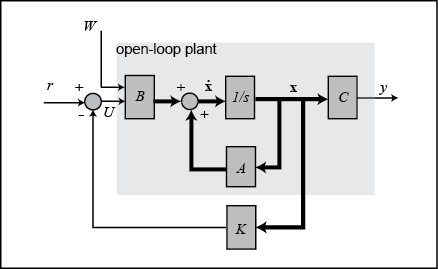
\includegraphics[width=0.4\textwidth]{stfb.png}
	\caption{Full state feedback block diagram. \cite{controltutorials}
	}
	\label{fig:stfb}
\end{figure}

Assuming no tracking $(r=0)$ and no external disturbance $(w=0)$, the system input is given by:

\begin{align*}
	u &= -Kx \\
	\dot{x} &= Ax - BKx \\
	\dot{x} &= x(A - BK) 
\end{align*}

\newpage
\section{Linear Quadratic regulator}
\subsection{Overview}
LQR controller is a widely used type of state feedback control that offers a systematic method for determining the control gain, $K$. The LQR approach will be employed in the controller design for the active suspension system, as it is a classic and straightforward option for linear, time-invariant, multiple-input multiple-output (MIMO) systems. One of the key advantages of using an LQR controller is its ability to weight the factors affecting the performance index based on the desired outcome. For this project, the focus of the LQR approach will be on enhancing ride comfort and improving road-handling performance in the quarter-car model.

The function of an LQR controller is to minimize the cost function, J, which is shown in the following equation:

\begin{equation}
	J = \frac{1}{2} \int_{0}^{t} (x^{T}Qx + u^{T}Ru) \, dt 
\end{equation}

$x^{T}$ = State vector.\\

$u^{T}$ = Input vector.

\subsection{LQR Implementation}
The weighting matrices, Q and R, within the quadratic performance index significantly influence the LQR controller's behavior. These matrices allow for tuning the control system's priorities, such as emphasizing ride comfort or minimizing control effort. The optimal values for Q and R were determined through iterative simulations and tuning within the MATLAB environment. This process involved systematically adjusting the elements of Q and R and observing the resulting system response to determine the combination that best met the desired performance objectives.\\ 

The following figure\ref{fig:lqr-final} shows the model used to simulate the dynamics of the quarter car suspension system, based on the state space model represented in the previous chapter. 

        \begin{figure}[H]
	\centering
	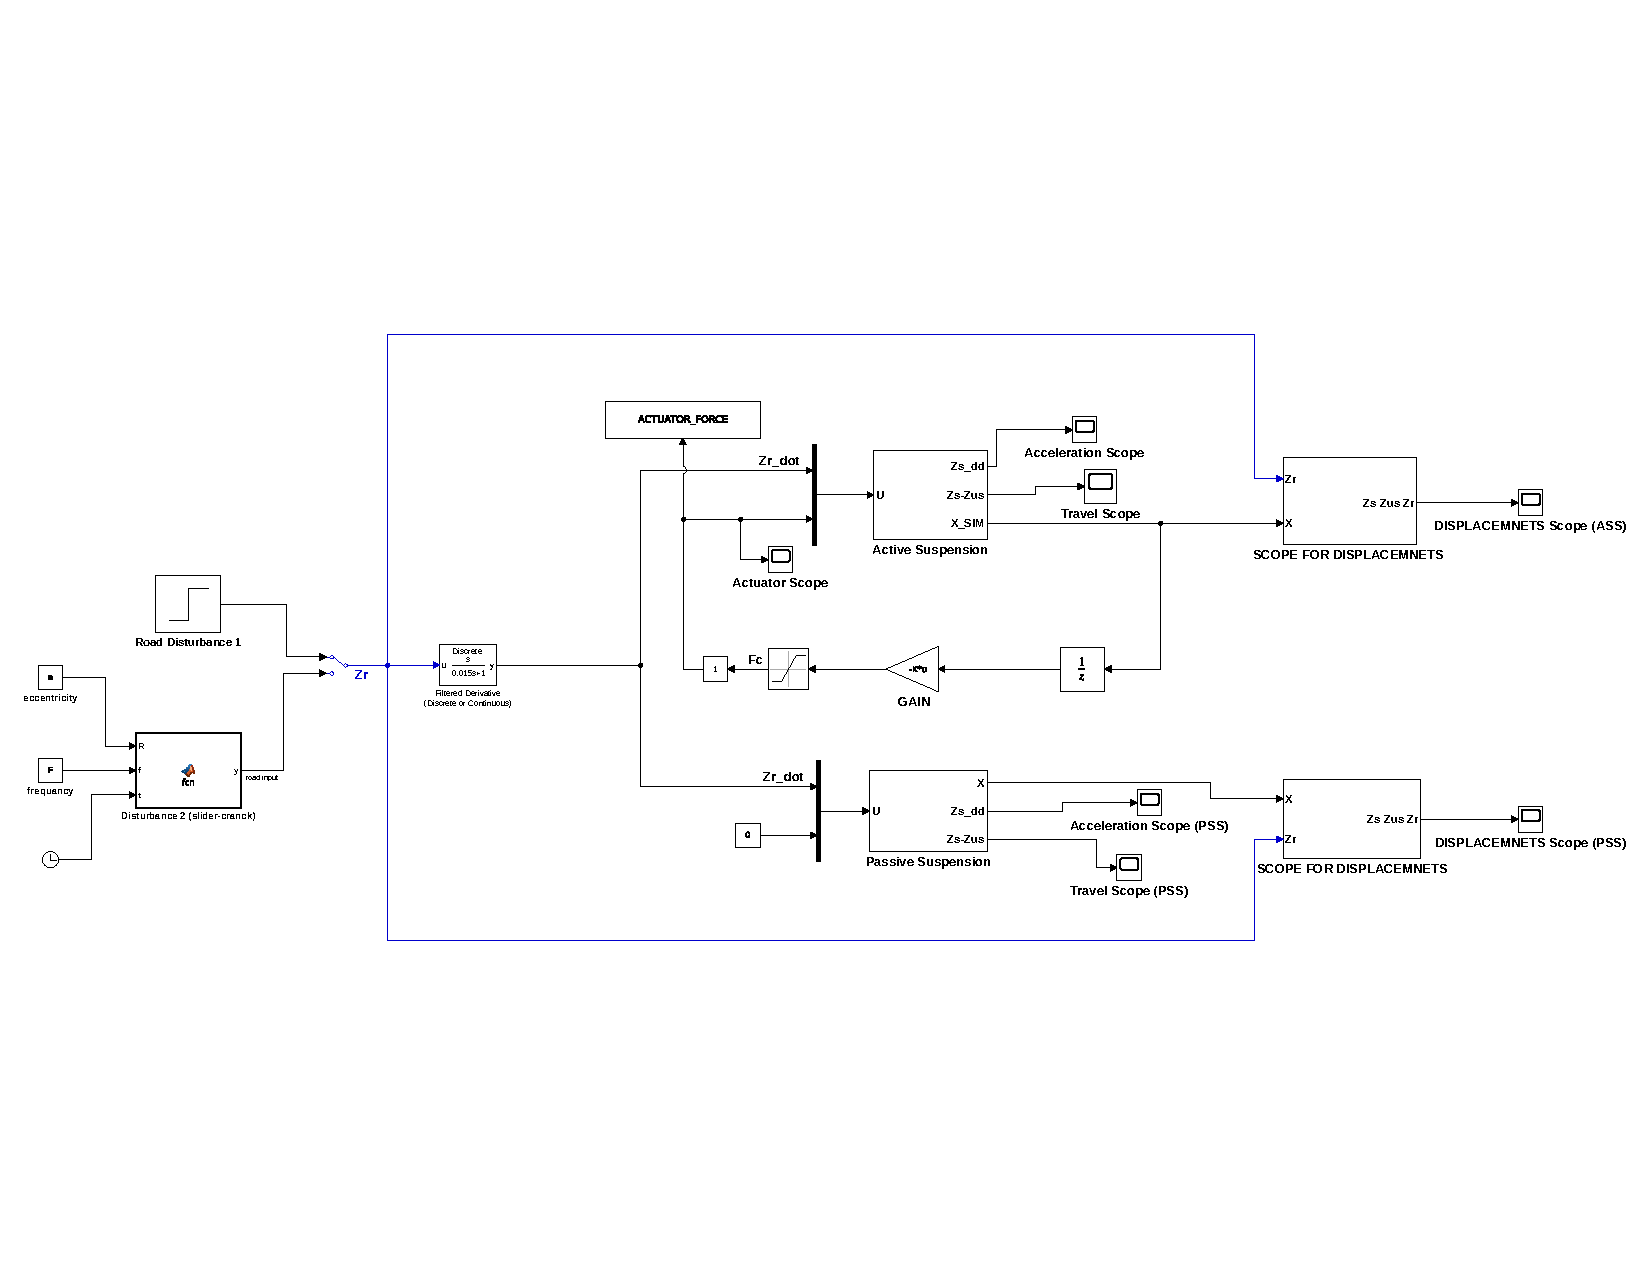
\includegraphics[trim=0cm 5cm 0cm 5cm, clip, width=1\linewidth]{figures/lqr-final.pdf}
	\caption{provides the block diagram model for the active suspension system}
	\label{fig:lqr-final}
\end{figure}

\newpage
\section{LQR Simulation Results}
To evaluate the performance of the LQR controller we will compare between the passive suspension system and the active suspension sytem in case of two road excitation profiles, the first one will be a simple step input, the second one will be the profile of the slider crank mechanism, that we discussed in the previous chapter (section 3.3)

\subsection{Step Response}
The following figure\ref{fig:step-sprungs} shows the effect of LQR on the system, it is a comparison between the passive and active response when excited by a step input of 60 mm amplitude.
 \begin{figure}[H]
	\centering
	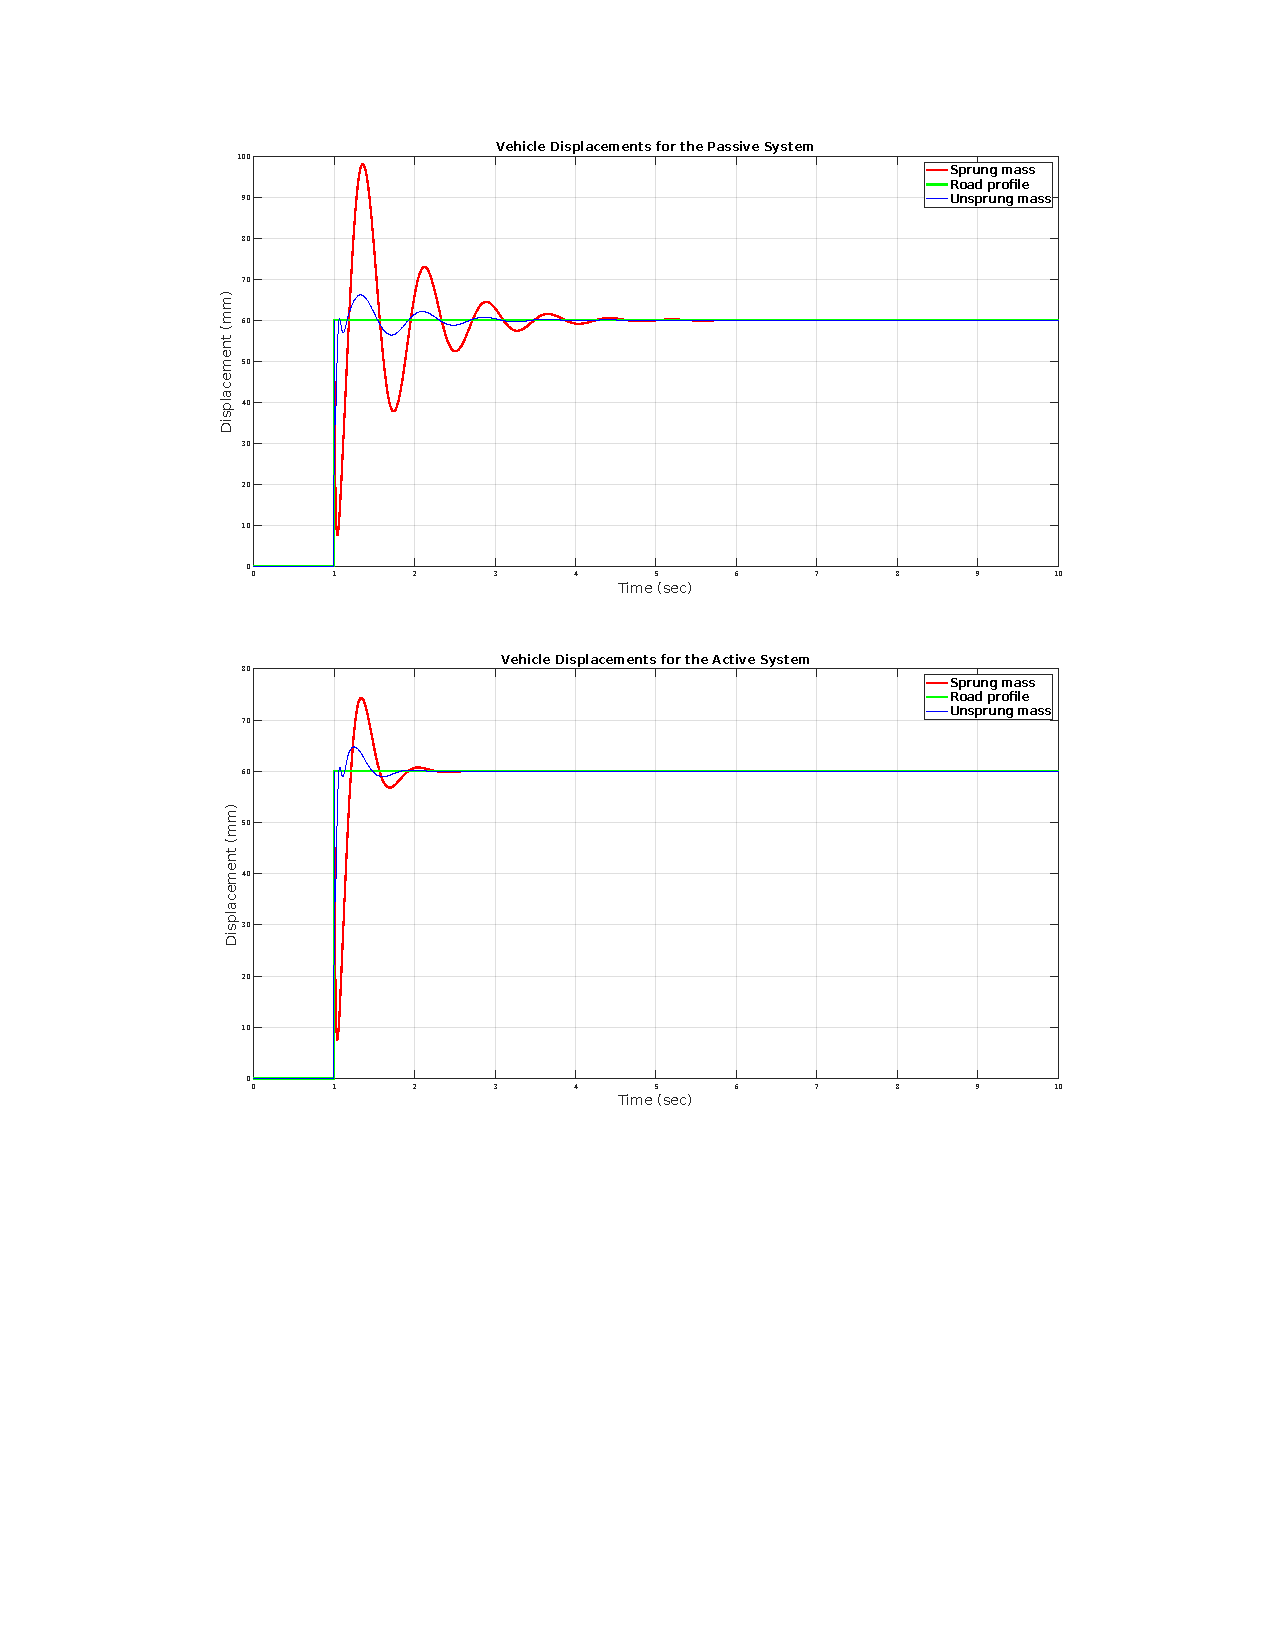
\includegraphics[trim=0cm 8cm 0cm 2cm, clip, width=1\linewidth]{figures/sprung-masses.pdf}
	\caption{Effect of the controller on Sprung and unsprung mass of the system}
	\label{fig:step-sprungs}
\end{figure}

\newpage
The following figures\ref{fig:all-step} compare between the performance of the system with LQR and without it to a step input: 
\begin{figure}[H]
	\centering
	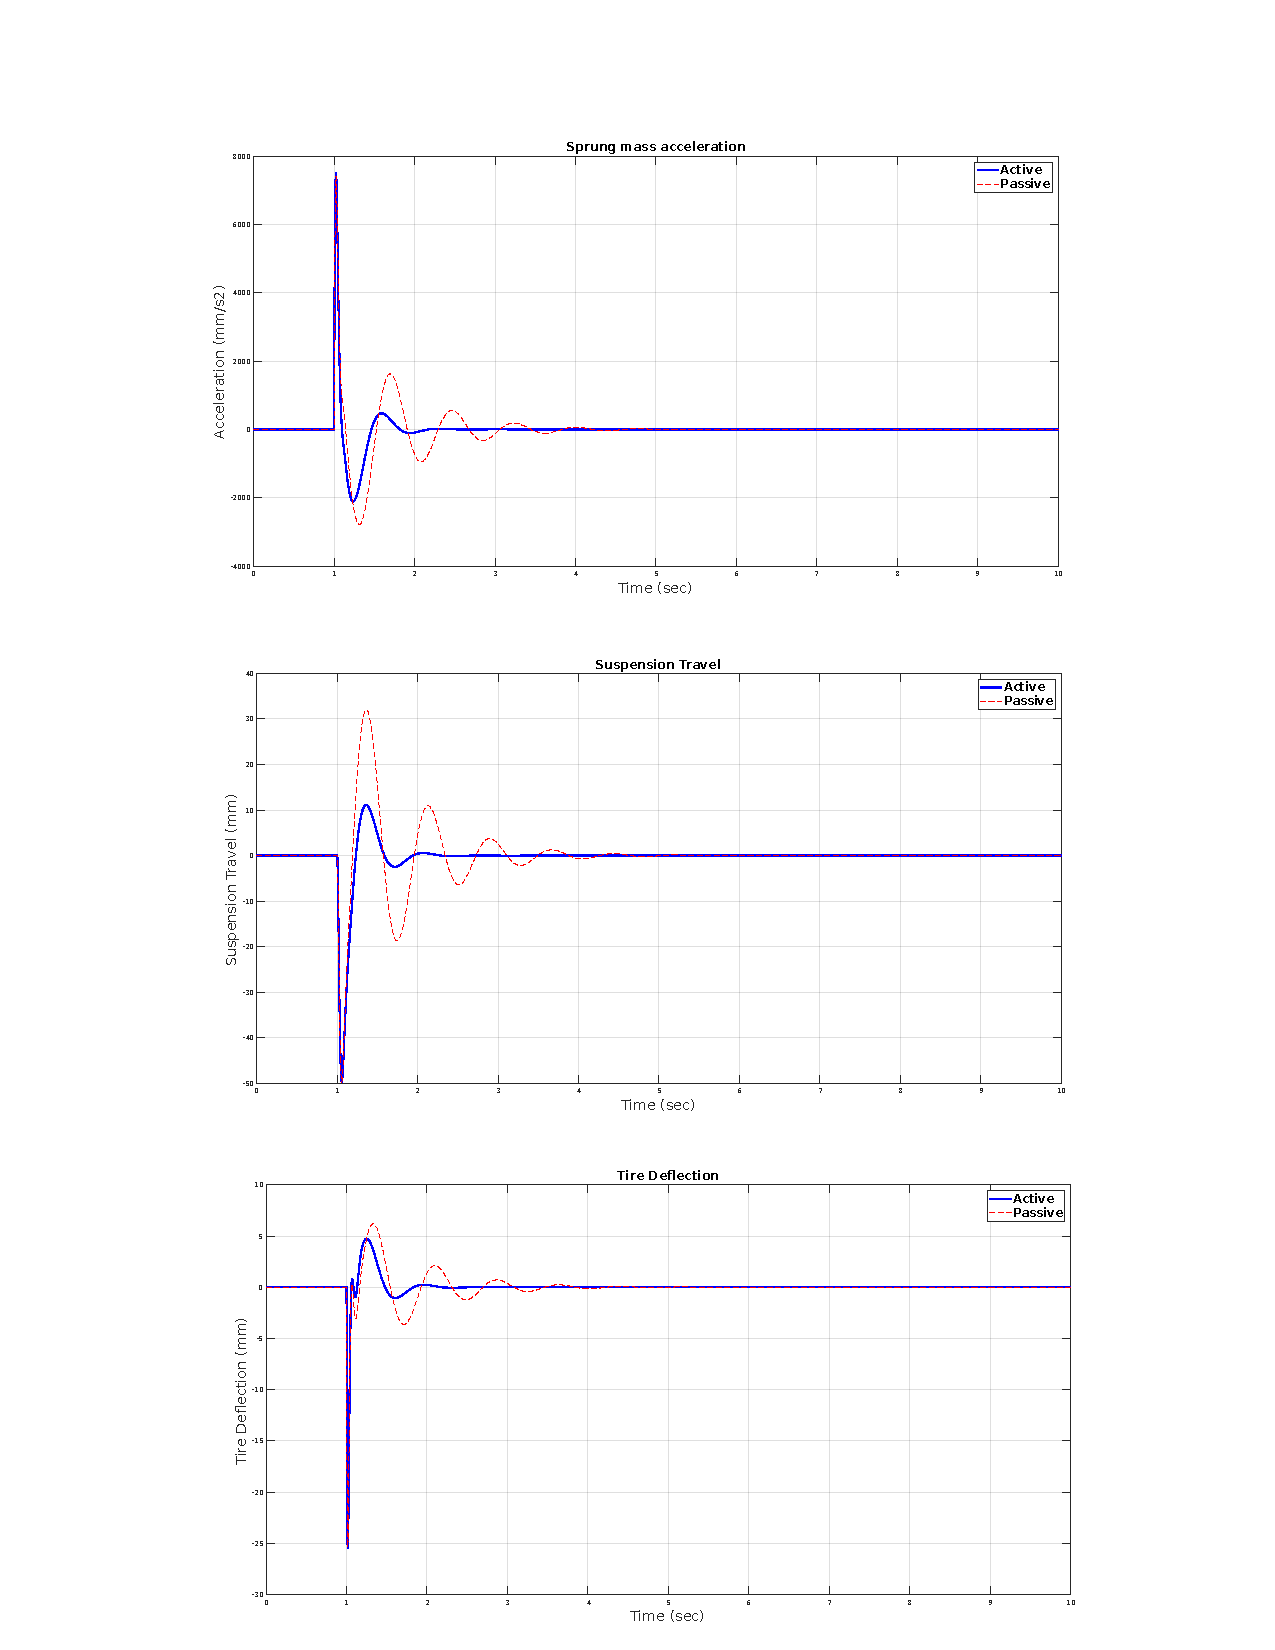
\includegraphics[trim=0cm 0cm 0cm 2cm, clip, width=1\linewidth]{figures/p-a-step.pdf}
	\caption{Effect of the controller}
	\label{fig:all-step}
\end{figure}

\newpage
\subsection{Road Profile Excitation}
This section shows the effect of the controller on the system against a more complicated road disturbance, which is the continuous excitation of the slider crank mechanism at a frequency of 0.3 HZ.

The following figures\ref{fig:road-sprungs} compare between the sprung and unsprung mass acceleration in both the passive and active systems:

 \begin{figure}[H]
	\centering
	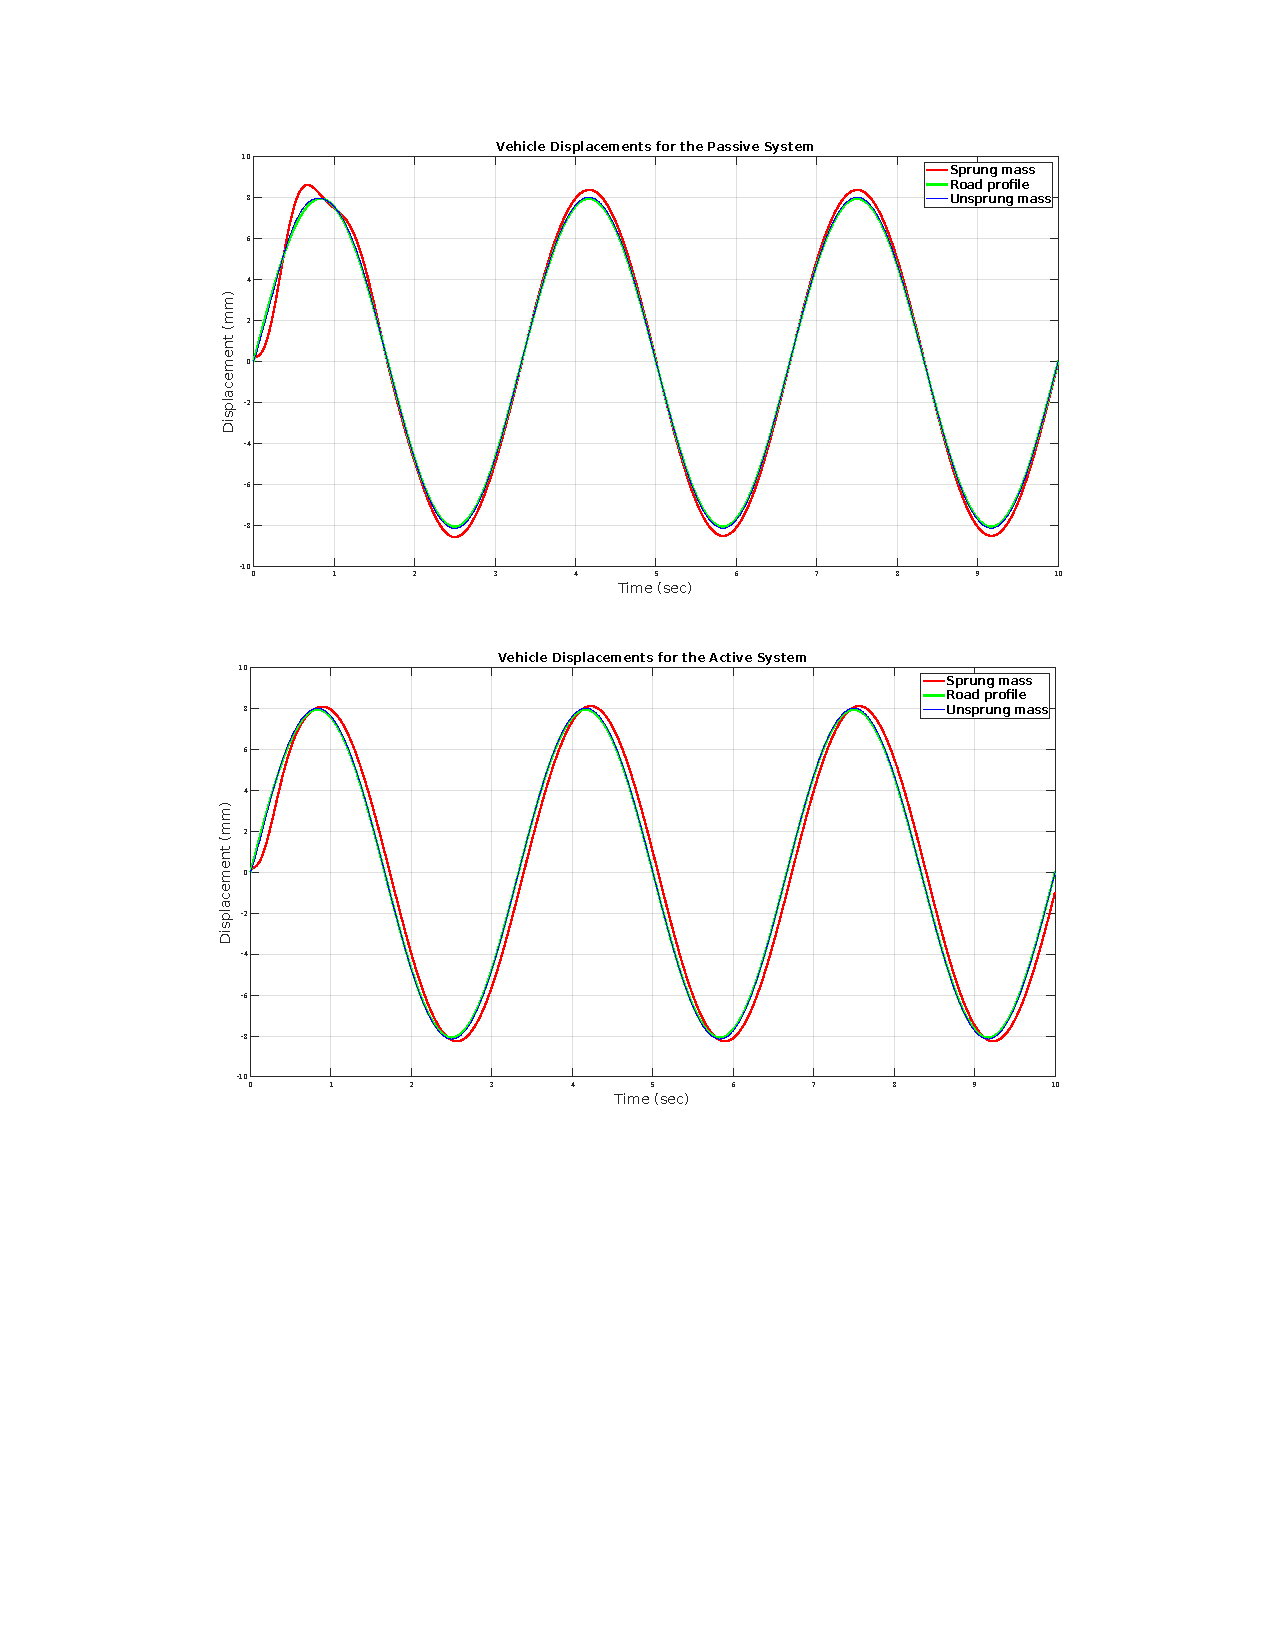
\includegraphics[trim=0cm 9cm 0cm 2cm, clip, width=1\linewidth]{figures/road-sprungs.pdf}
	\caption{Effect of the controller on Sprung and unsprung mass of the system}
	\label{fig:road-sprungs}
\end{figure}

\newpage
The following figures\ref{fig:all-road} compare between the performance of the system with LQR and without it, against the excitation of the road profile:
\begin{figure}[H]
	\centering
	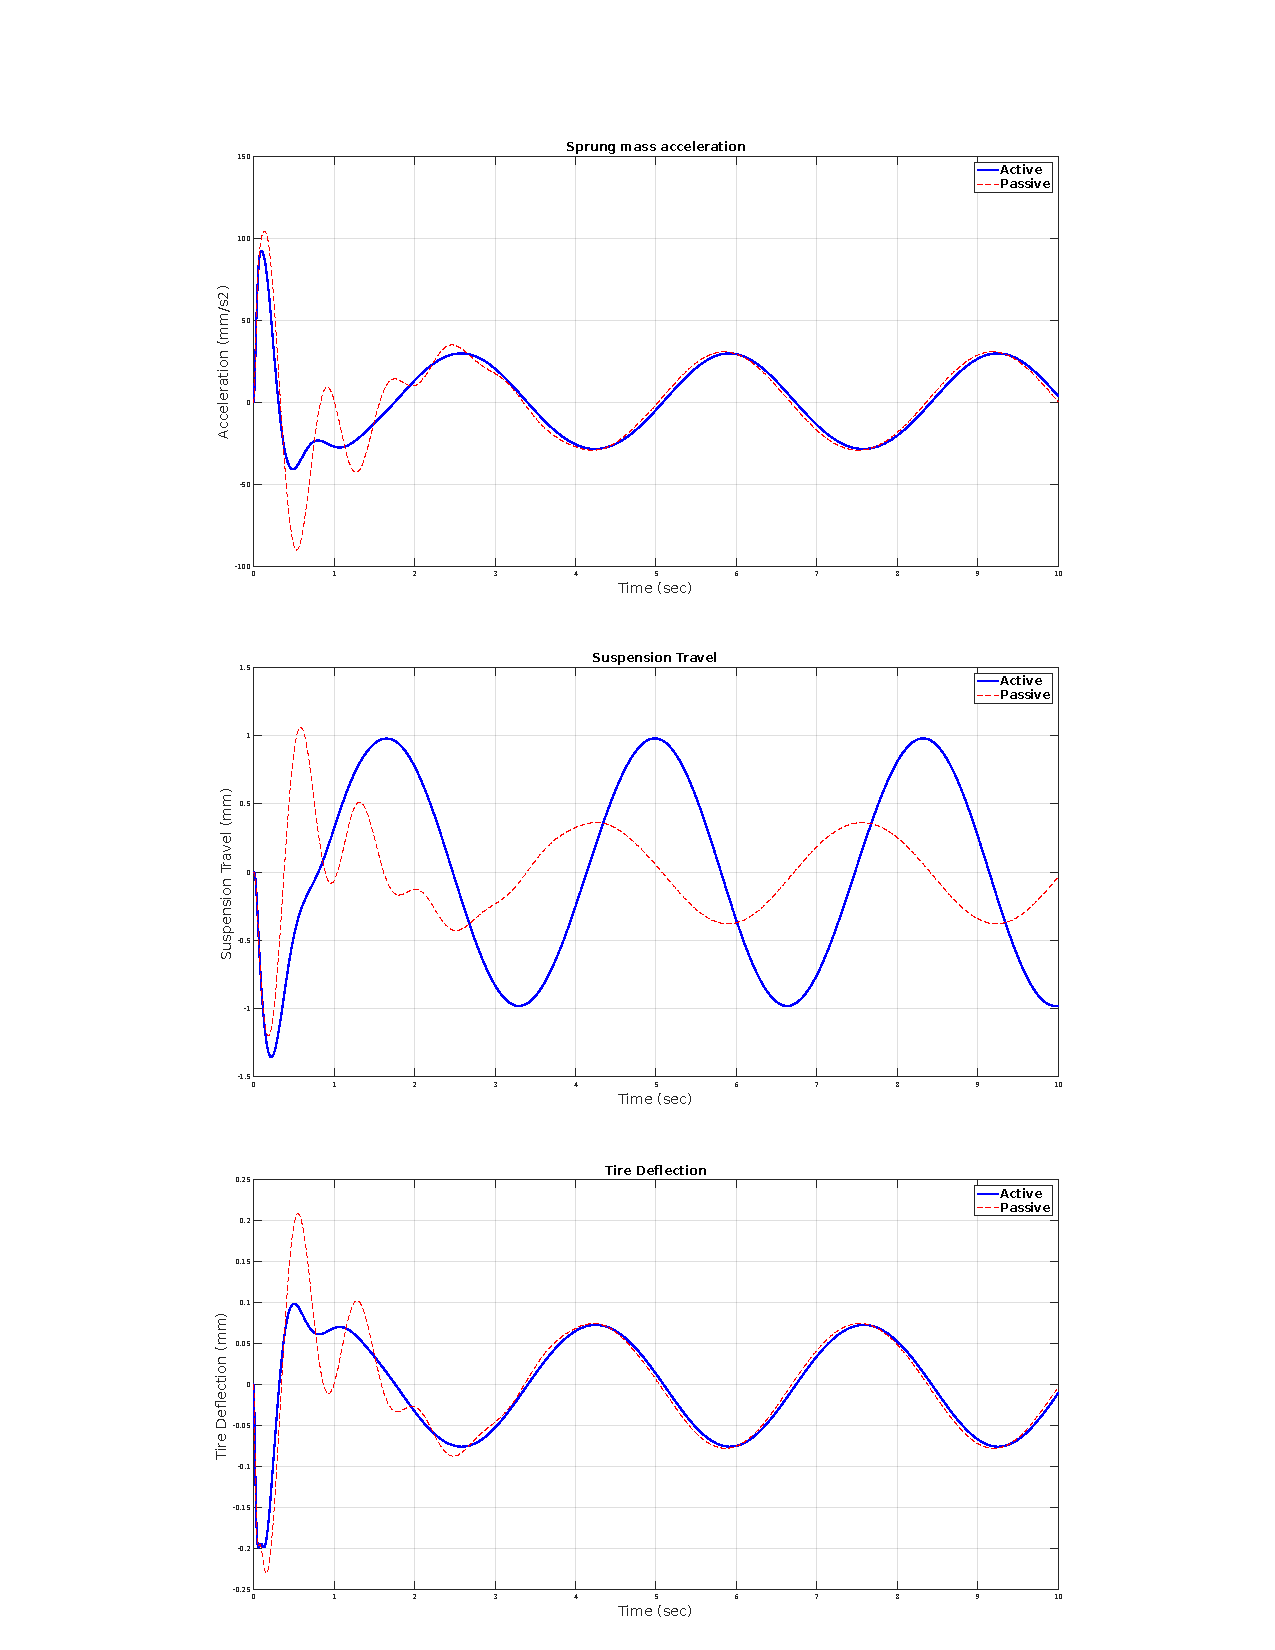
\includegraphics[trim=0cm 1cm 0cm 2cm, clip, width=1\linewidth]{figures/p-a-road.pdf}
	\caption{Effect of the controller}
	\label{fig:all-road}
\end{figure}

\newpage
\section{Sliding mode control}
\subsection{Overview}
Sliding Mode Control (SMC) is a nonlinear control technique featuring
remarkable properties of accuracy, robustness, and easy tuning and implementation. There are
two main advantages of sliding mode control. First is that the dynamic behavior of the system may
be tailored by the particular choice of the sliding function. Secondly, the closed loop response
becomes totally insensitive to some particular uncertainties. This principle extends to model
parameter uncertainties, disturbance and non-linearity that are bounded. From a practical point
of view (SMC) allows for controlling nonlinear processes subject to external disturbances and
model uncertainties
\subsection{Theory}
This is a type of non-linear control that provides a sporadic control signal in the process of altering dynamic characteristics of a system. The sliding mode control (SMC) is based on the principle of switching logic between different independent structural systems. The control strategy forces the system to slide along the normal behavioural lines. The control system is structured in such a way that paths always move towards a neighbouring region of the behavioural line with a different degree of control so that the ultimate path would not occur exclusively within one control. It will instead slide along the limits of the controlled structures while minimizing error, as indicated in \ref{fig:smc}. The SMC is, therefore, able to control both linear and non-linear systems. (1) The controller and (2) the sliding surface are the primary parameters of SMC.
\begin{figure}[H]
	\centering
	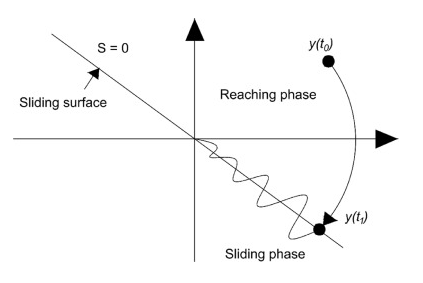
\includegraphics[width=0.4\textwidth]{SMC_theory.png}
	\caption{Representation of sliding surface and minimization of error. \cite{WANI2022103}
	} \label{fig:smc}
\end{figure}
\subsection{SMC implementation}
Using regulation mode to minimize system vibrations and improve ride comfort the first step is to define the sliding surface 
\subsubsection{Dfinning the sliding surface}
The sliding surface (or switching surface) is a key component of the SMC. It defines the condition under which the system behavior will enter a "sliding" mode. The sliding-mode surface can be described as:
\begin{equation}
	s = cZ_s+\dot{Z_s}
\end{equation}

\subsubsection{Design reaching law}
The reaching law ensures that the state of the system moves towards the sliding surface whatever its initial conditions. The reaching law is given by:
\begin{equation}
	h\left(s\left(x\right)\right) = -\eta sign\left(s\right)
\end{equation}
where $\eta$ is a positive constant that determines the speed of convergence to the sliding surface.

\newpage
\subsubsection{Design the control law}
The sliding mode control law is designed to drive the system towards the sliding surface.
The derivative of s is given by:
\begin{equation}
	\dot{s} = c\dot{Z_s}+\ddot{Z_s}
	\label{equ:43}
\end{equation}
From mathematical model equation the sprung mass acceleration is given by:
\begin{equation}
	\ddot{Z}_s = \frac{B_s\dot{Z}_{us}}{M_s} - \frac{B_s\dot{Z}_s}{M_s} - \frac{K_s(Z_s - Z_{us})}{M_s} + \frac{1}{M_s}F_c
\end{equation}
substitute in \ref{equ:43} :
\begin{equation}
	\dot{s} = c\dot{Z_s}-\frac{K_s}{M_s}Z_s + \frac{K_s}{M_s}Z_us + \frac{1}{M_s}F_c
\end{equation}
Let $\dot{s} = -\eta sign\left(s\right) $
\begin{equation}
	-\eta sign\left(s\right)= c\dot{Z_s}-\frac{K_s}{M_s}Z_s + \frac{K_s}{M_s}Z_us + \frac{1}{M_s}F_c
\end{equation}
Therefore, sliding-mode control input is given by :
\begin{equation}
	F_c= -cM_s\dot{Z_s}+K_sZ_s - K_sZ_us -\eta M_s sign\left(s\right)
\end{equation}
\subsubsection{Define boundary layer}
Using a saturation boundary layer instead of the sign function can effectively reduce the chattering effect. The idea is to apply the full gain when the system state is outside the boundary layer. However, once the system enters the boundary layer, the gain is made proportional to the distance from the boundary, effectively smoothing the control action. This modification ensures a continuous control signal within the boundary layer, mitigating chattering while maintaining robustness.
\begin{equation}
	\text{sat}(s, \phi) =
	\begin{cases} 
		1 & \text{if } s > \phi, \\
		\frac{s}{\phi} & \text{if } -\phi \leq s \leq \phi, \\
		-1 & \text{if } s < -\phi.
	\end{cases}
\end{equation}
After designing the control force to enhance the performance of the suspension system, the next step is to implement the Sliding Mode Controller (SMC) using MATLAB/Simulink.
\begin{figure}[H]
	\centering
	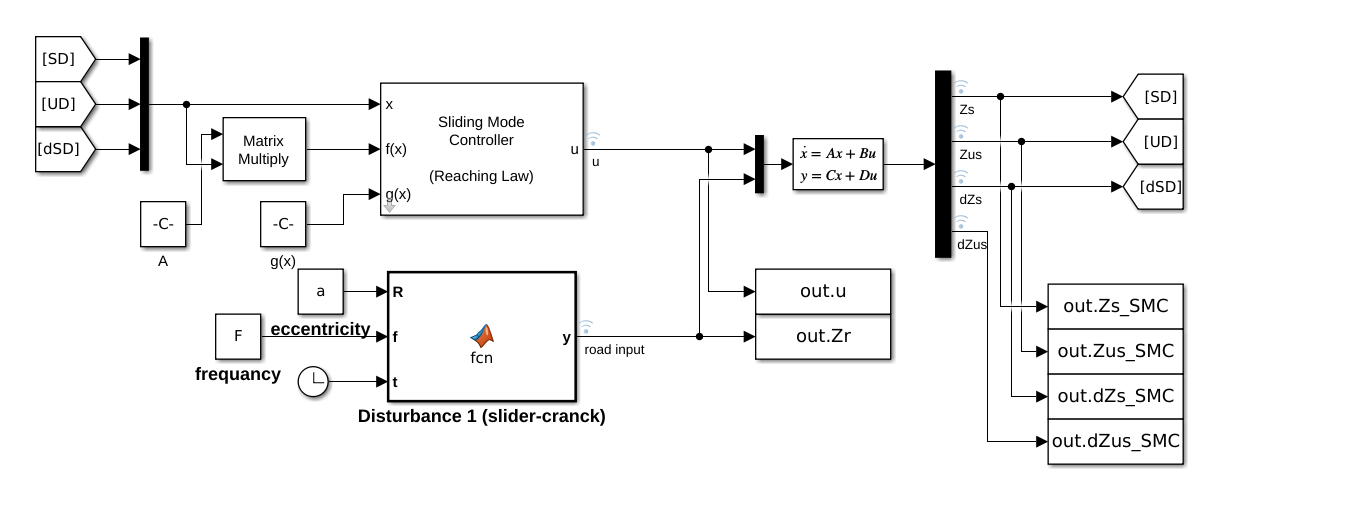
\includegraphics[width=1\textwidth]{SMC_simulink}
	\caption{SMC simulink model 
	}
\end{figure}

\newpage
\section{SMC Simulation Results}
The followinf figures shows the effect of the SMC on the suspension system when excited with the road profile defined by the slider crank mechanism:

Figure\ref{fig:smc1} shows the enhancement caused by SMC on the sprung mass, whicle figure  \ref{fig:smc2} shows the effect on the unsprung mass. Also the effect on suspension travel is shown in figure \ref{fig:smc3}.
\begin{figure}[H]
	\centering
	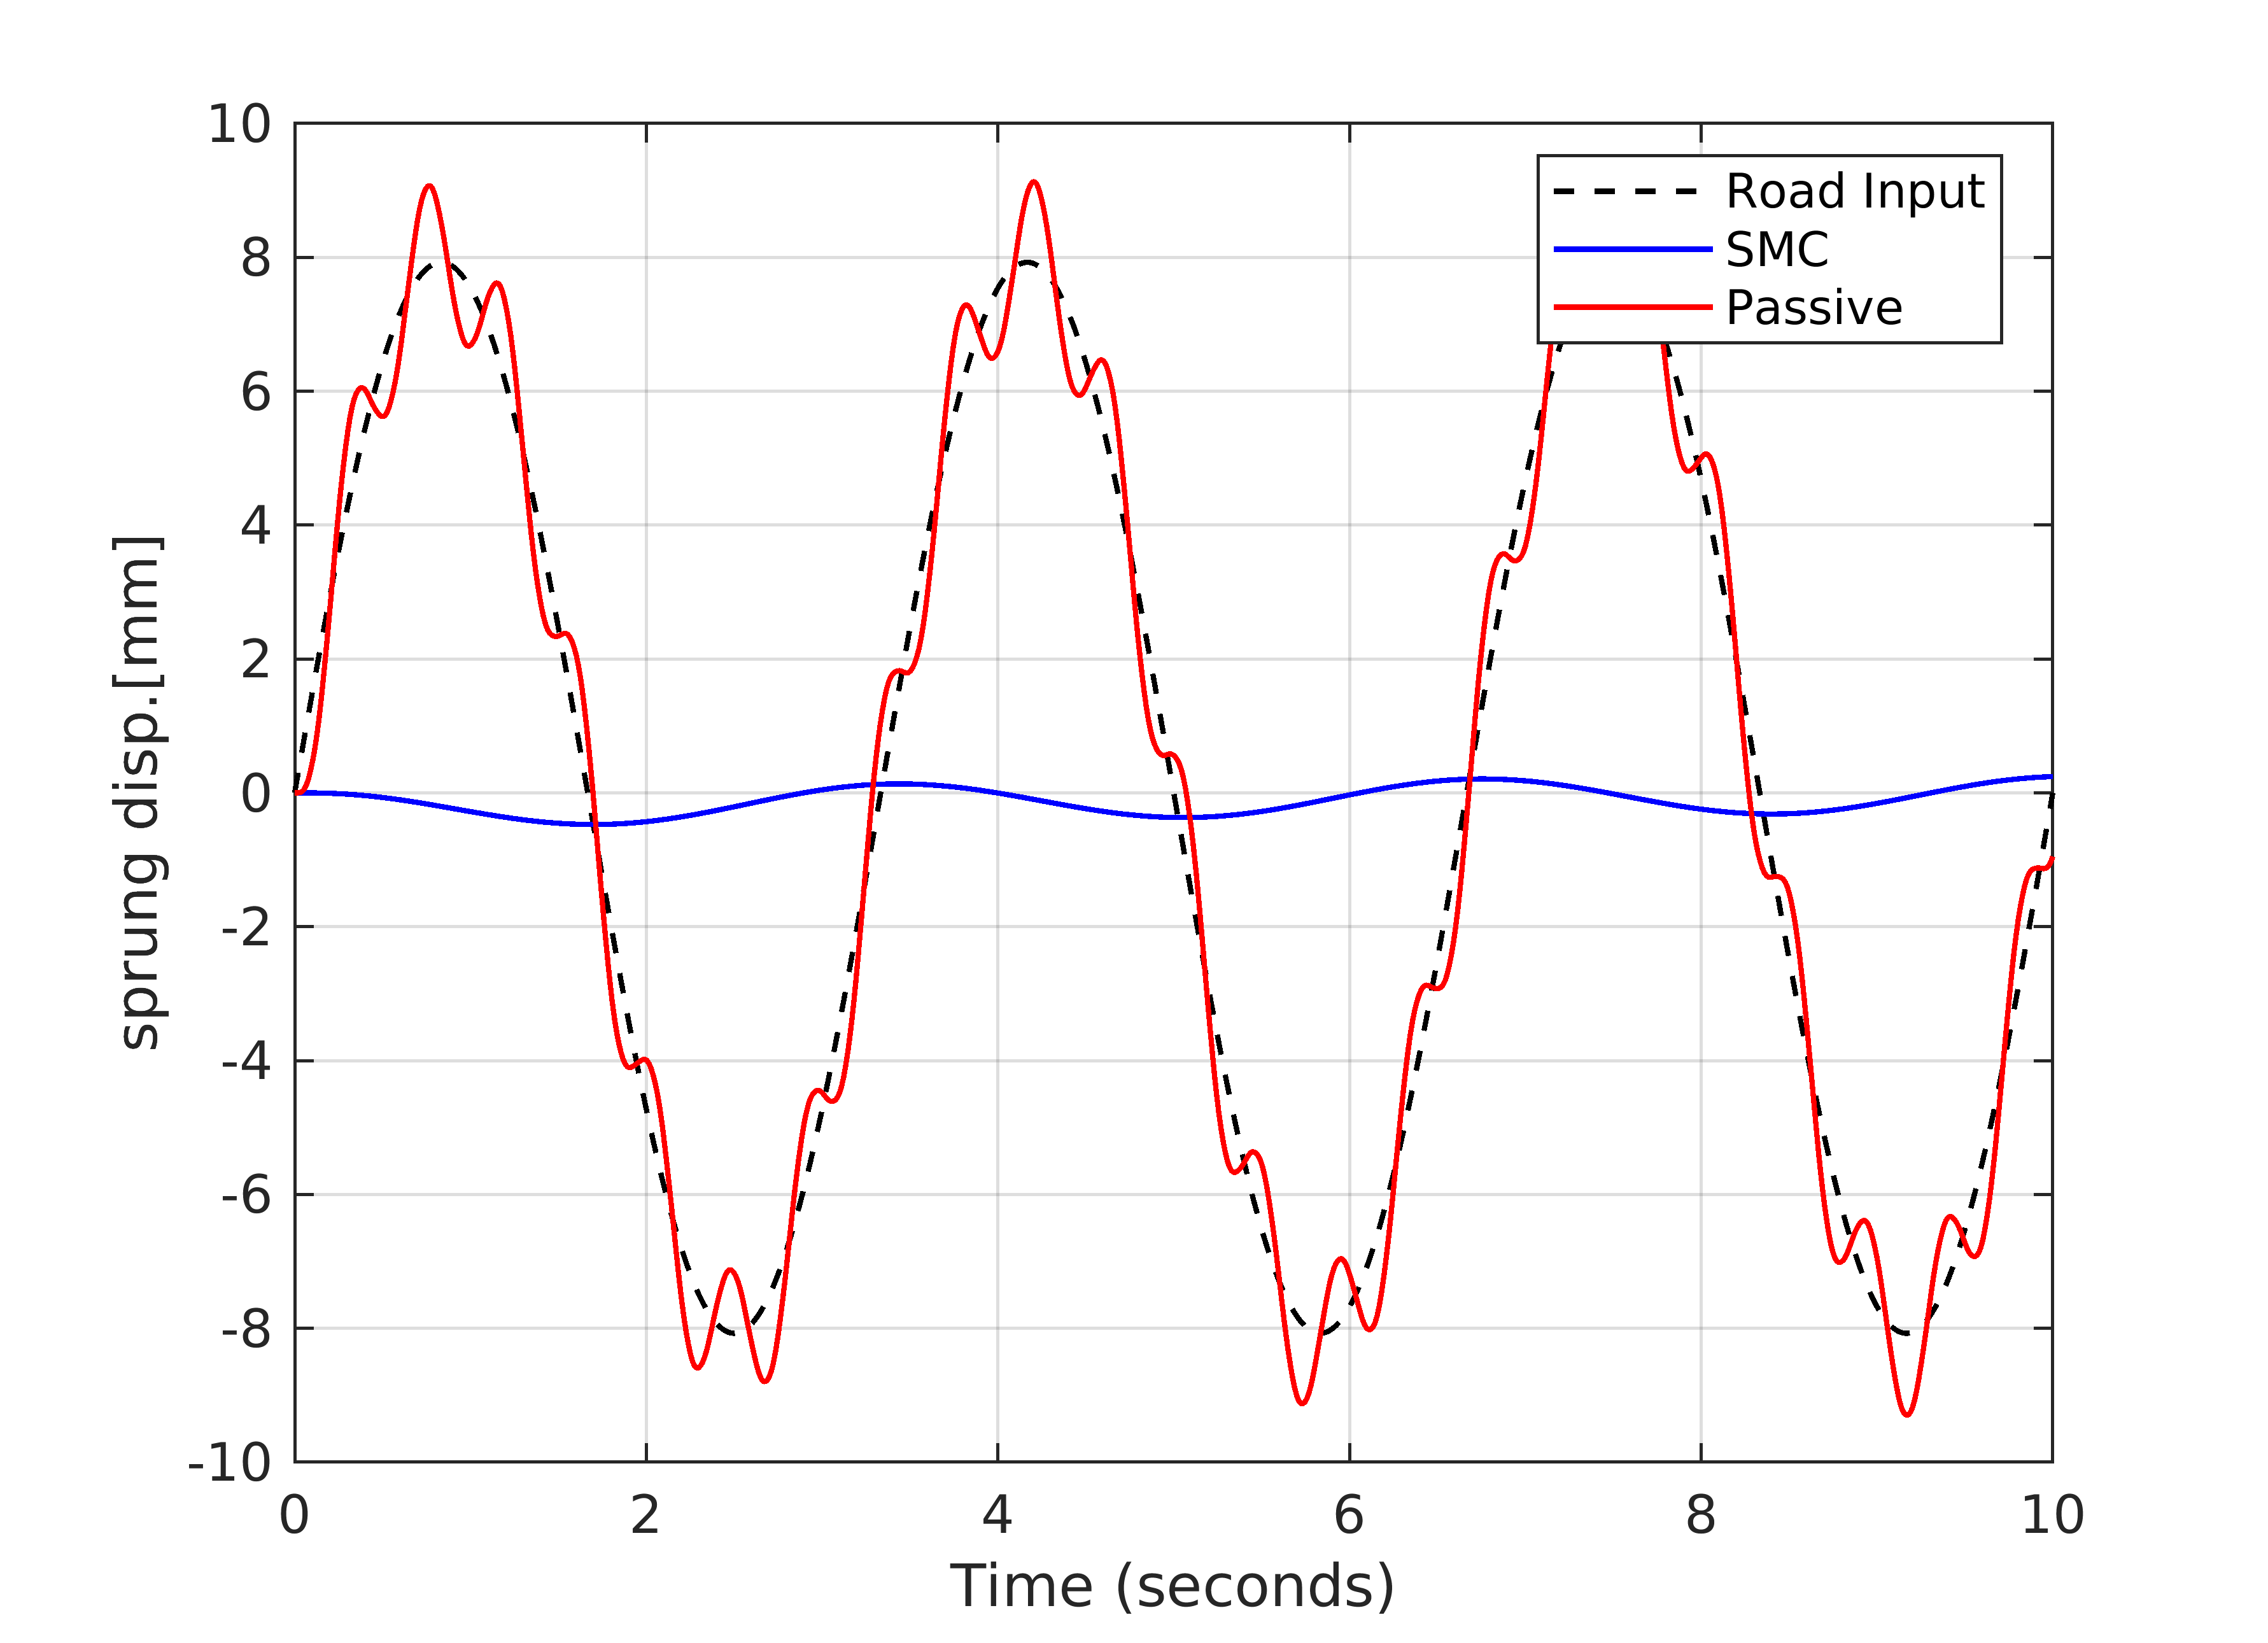
\includegraphics[trim=0cm 2cm 0cm 2cm, clip, width=0.5\textwidth]{SD}
	\caption{Sprung mass displacement. }
	\label{fig:smc1}
\end{figure}

\begin{figure}[H]
	\centering
	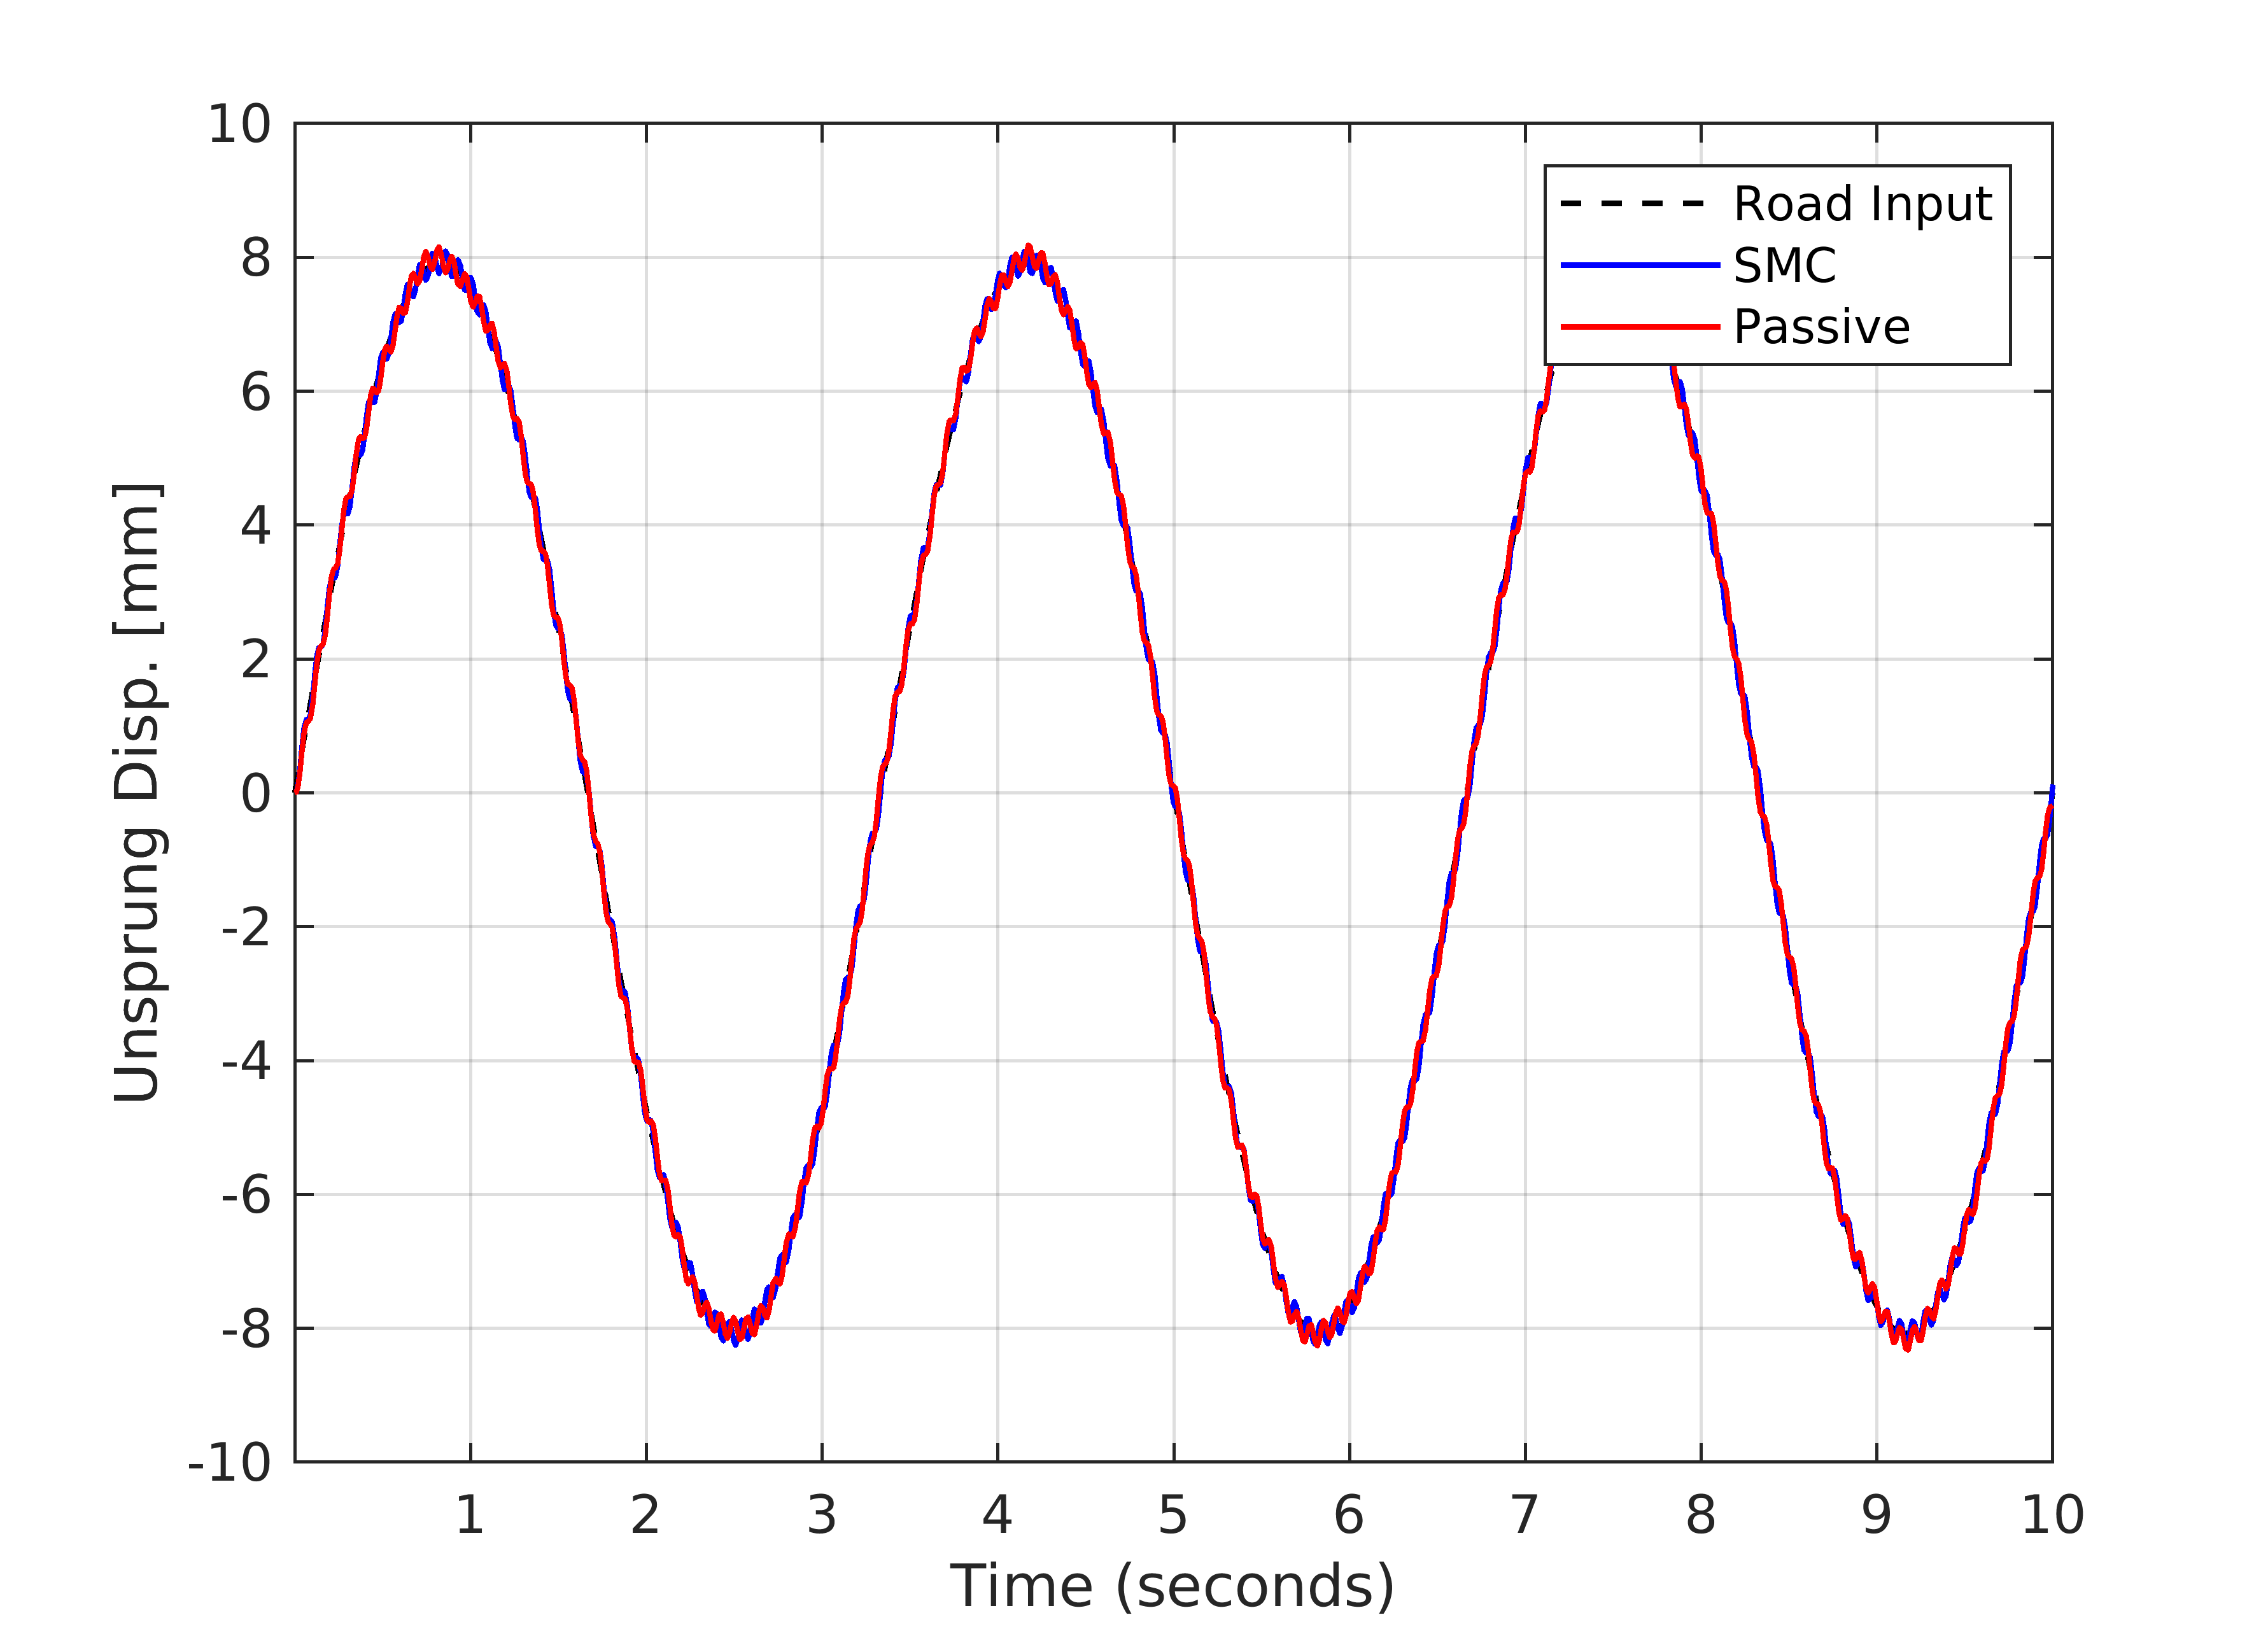
\includegraphics[trim=0cm 2cm 0cm 2cm, clip, width=0.5\textwidth]{usd}
	\caption{Usprung mass displacement. }
	\label{fig:smc2}
\end{figure}

\begin{figure}[H]
	\centering
	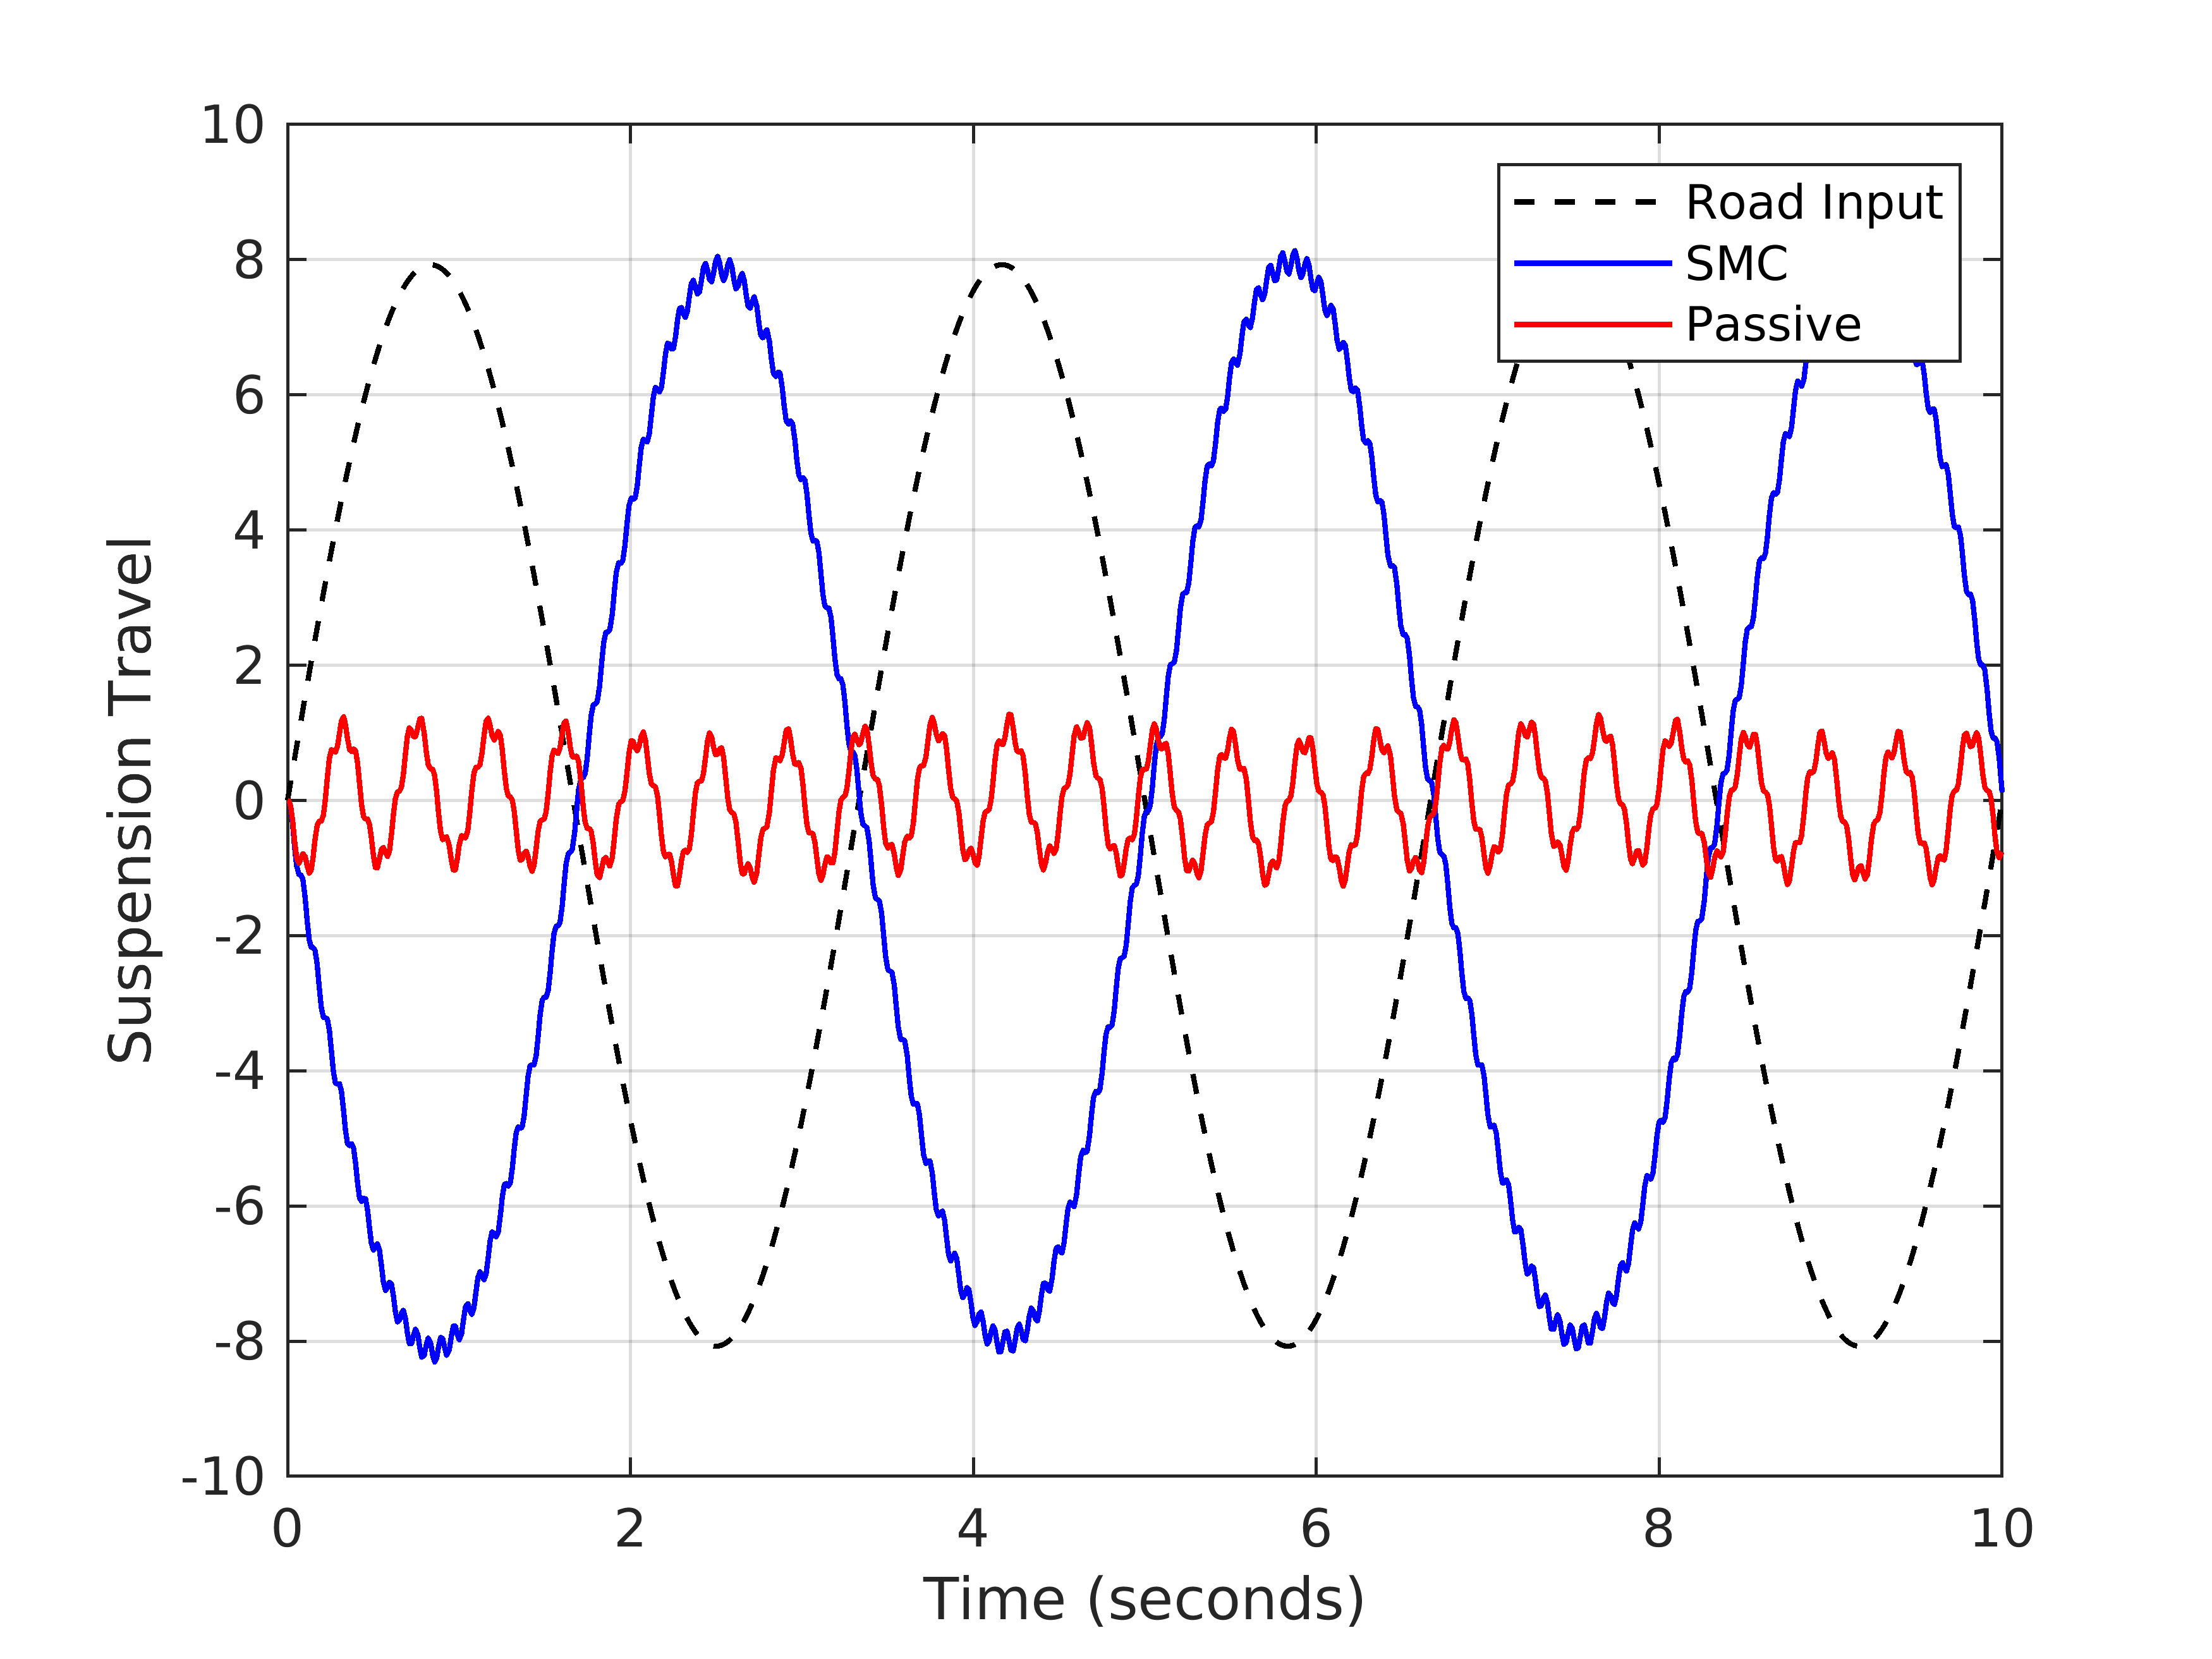
\includegraphics[trim=0cm 2cm 0cm 2cm, clip, width=0.5\textwidth]{sus t}
	\caption{Suspension travel. }
	\label{fig:smc3}
\end{figure}


\newpage
The following figure \ref{fig:smc4} shows the effect of the SMC on the tire deflection, while figure \ref{fig:smc5} shows the effect on sprung mass acceleration.

\begin{figure}[H]
	\centering
	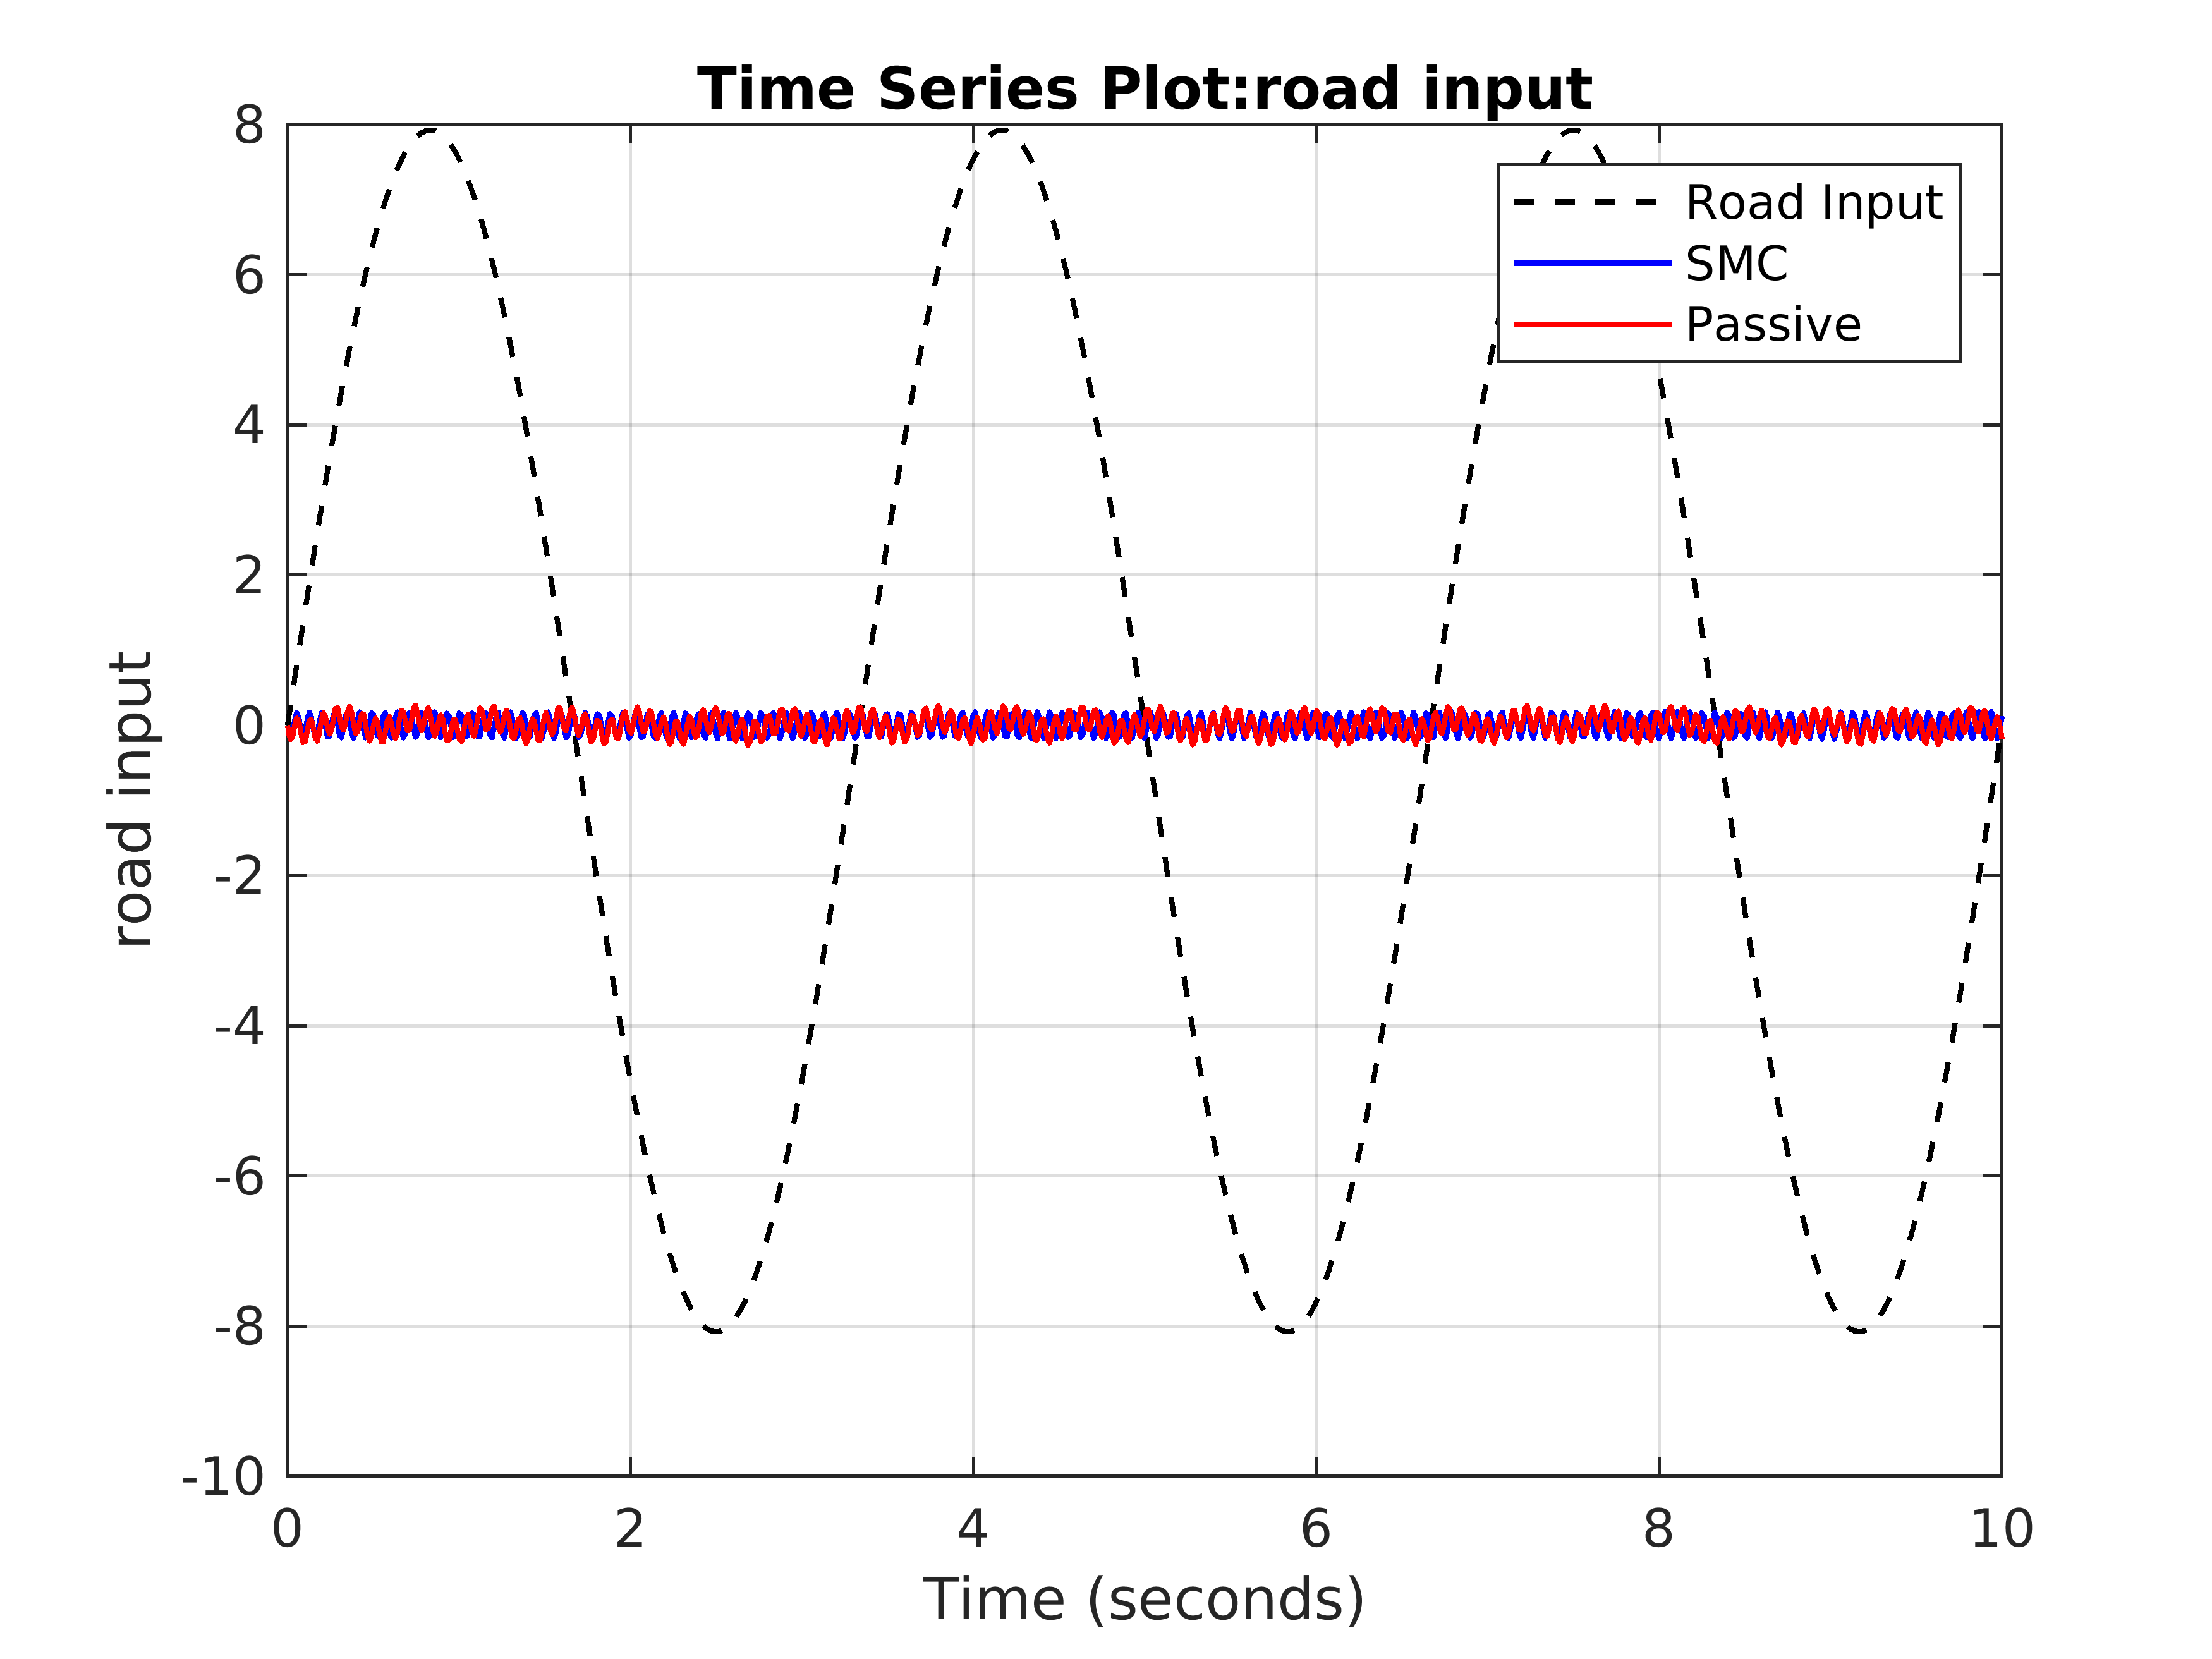
\includegraphics[trim=0cm 2cm 0cm 2cm, clip, width=0.5\textwidth]{TD}
	\caption{Dynamic tire defeliction. }
	\label{fig:smc4}
\end{figure}

\begin{figure}[H]
	\centering
	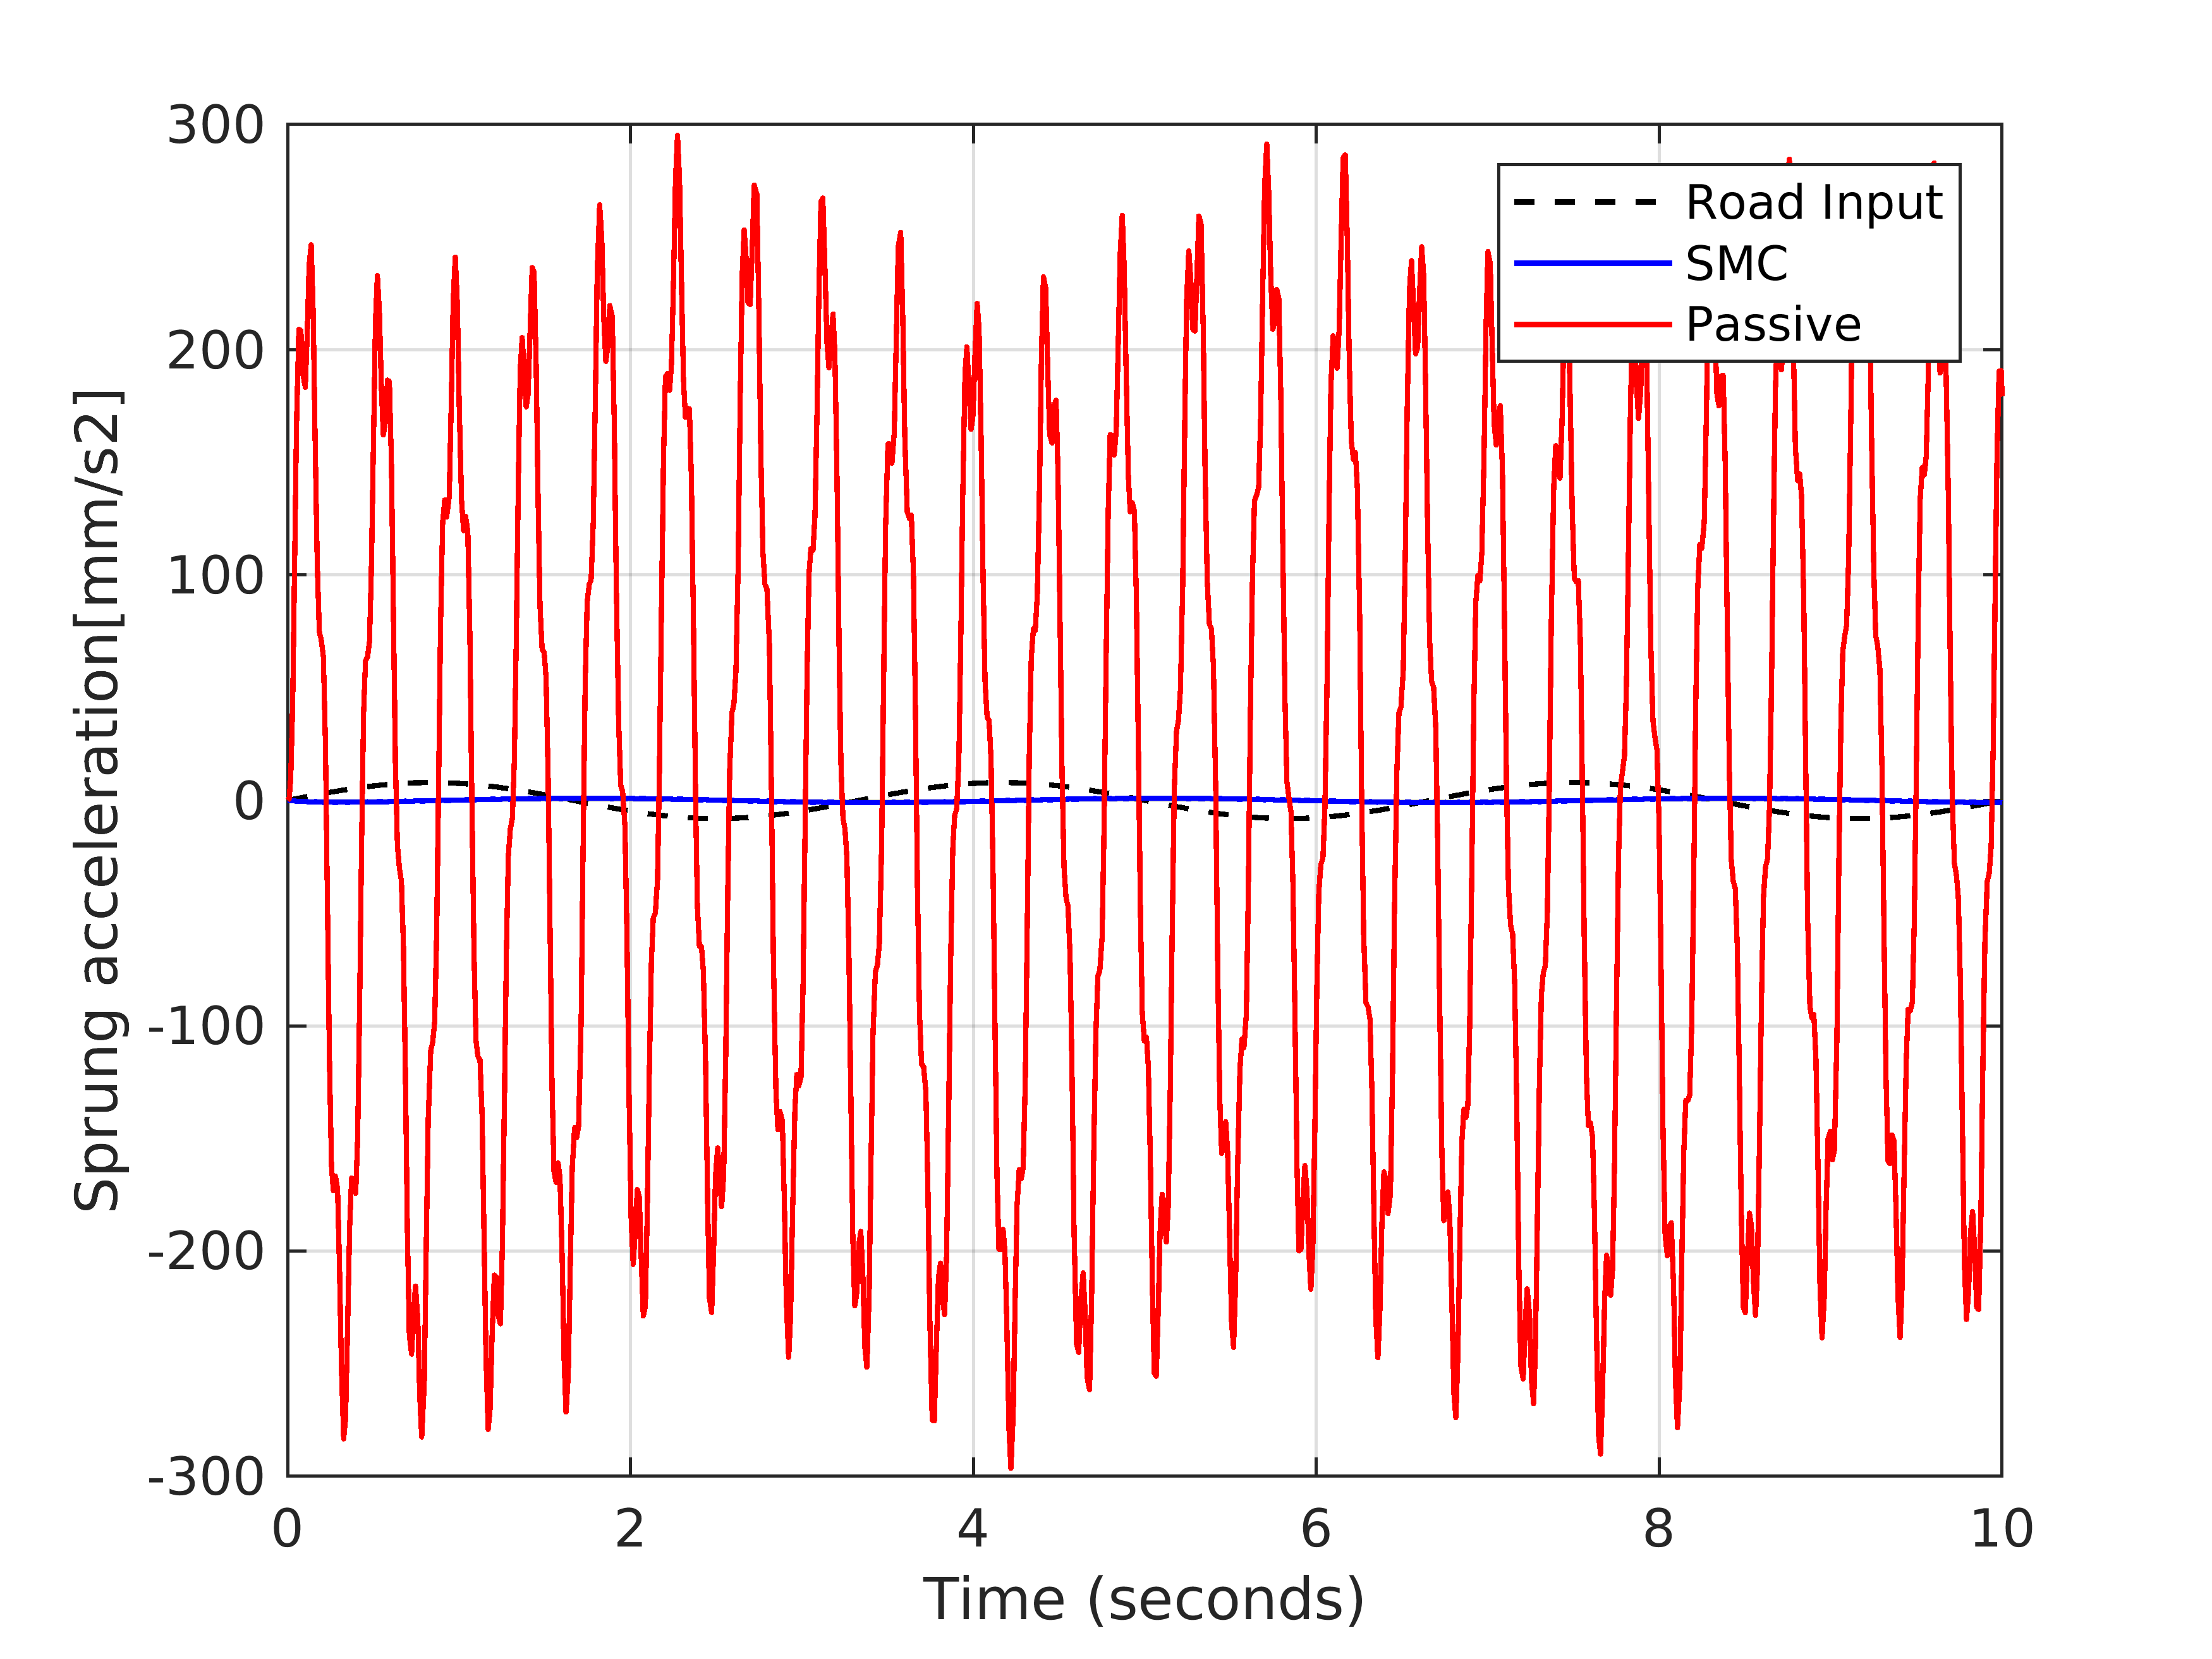
\includegraphics[trim=0cm 1.8cm 0cm 2cm, clip, width=0.5\textwidth]{accel}
	\caption{Sprung mass acceleration. }
	\label{fig:smc5}
\end{figure}

\subsection{Maximum Actuator force}
To ensure the practical feasibility and safety of the proposed control system, actuator limitations were carefully considered throughout the design process. A maximum force constraint of 100 Newtons was imposed on the actuator, which was deemed sufficient for all operating conditions, including the more demanding scenarios encountered with Sliding Mode Control as shown in figure \ref{fig:smc6}. 
\begin{figure}[H]
	\centering
	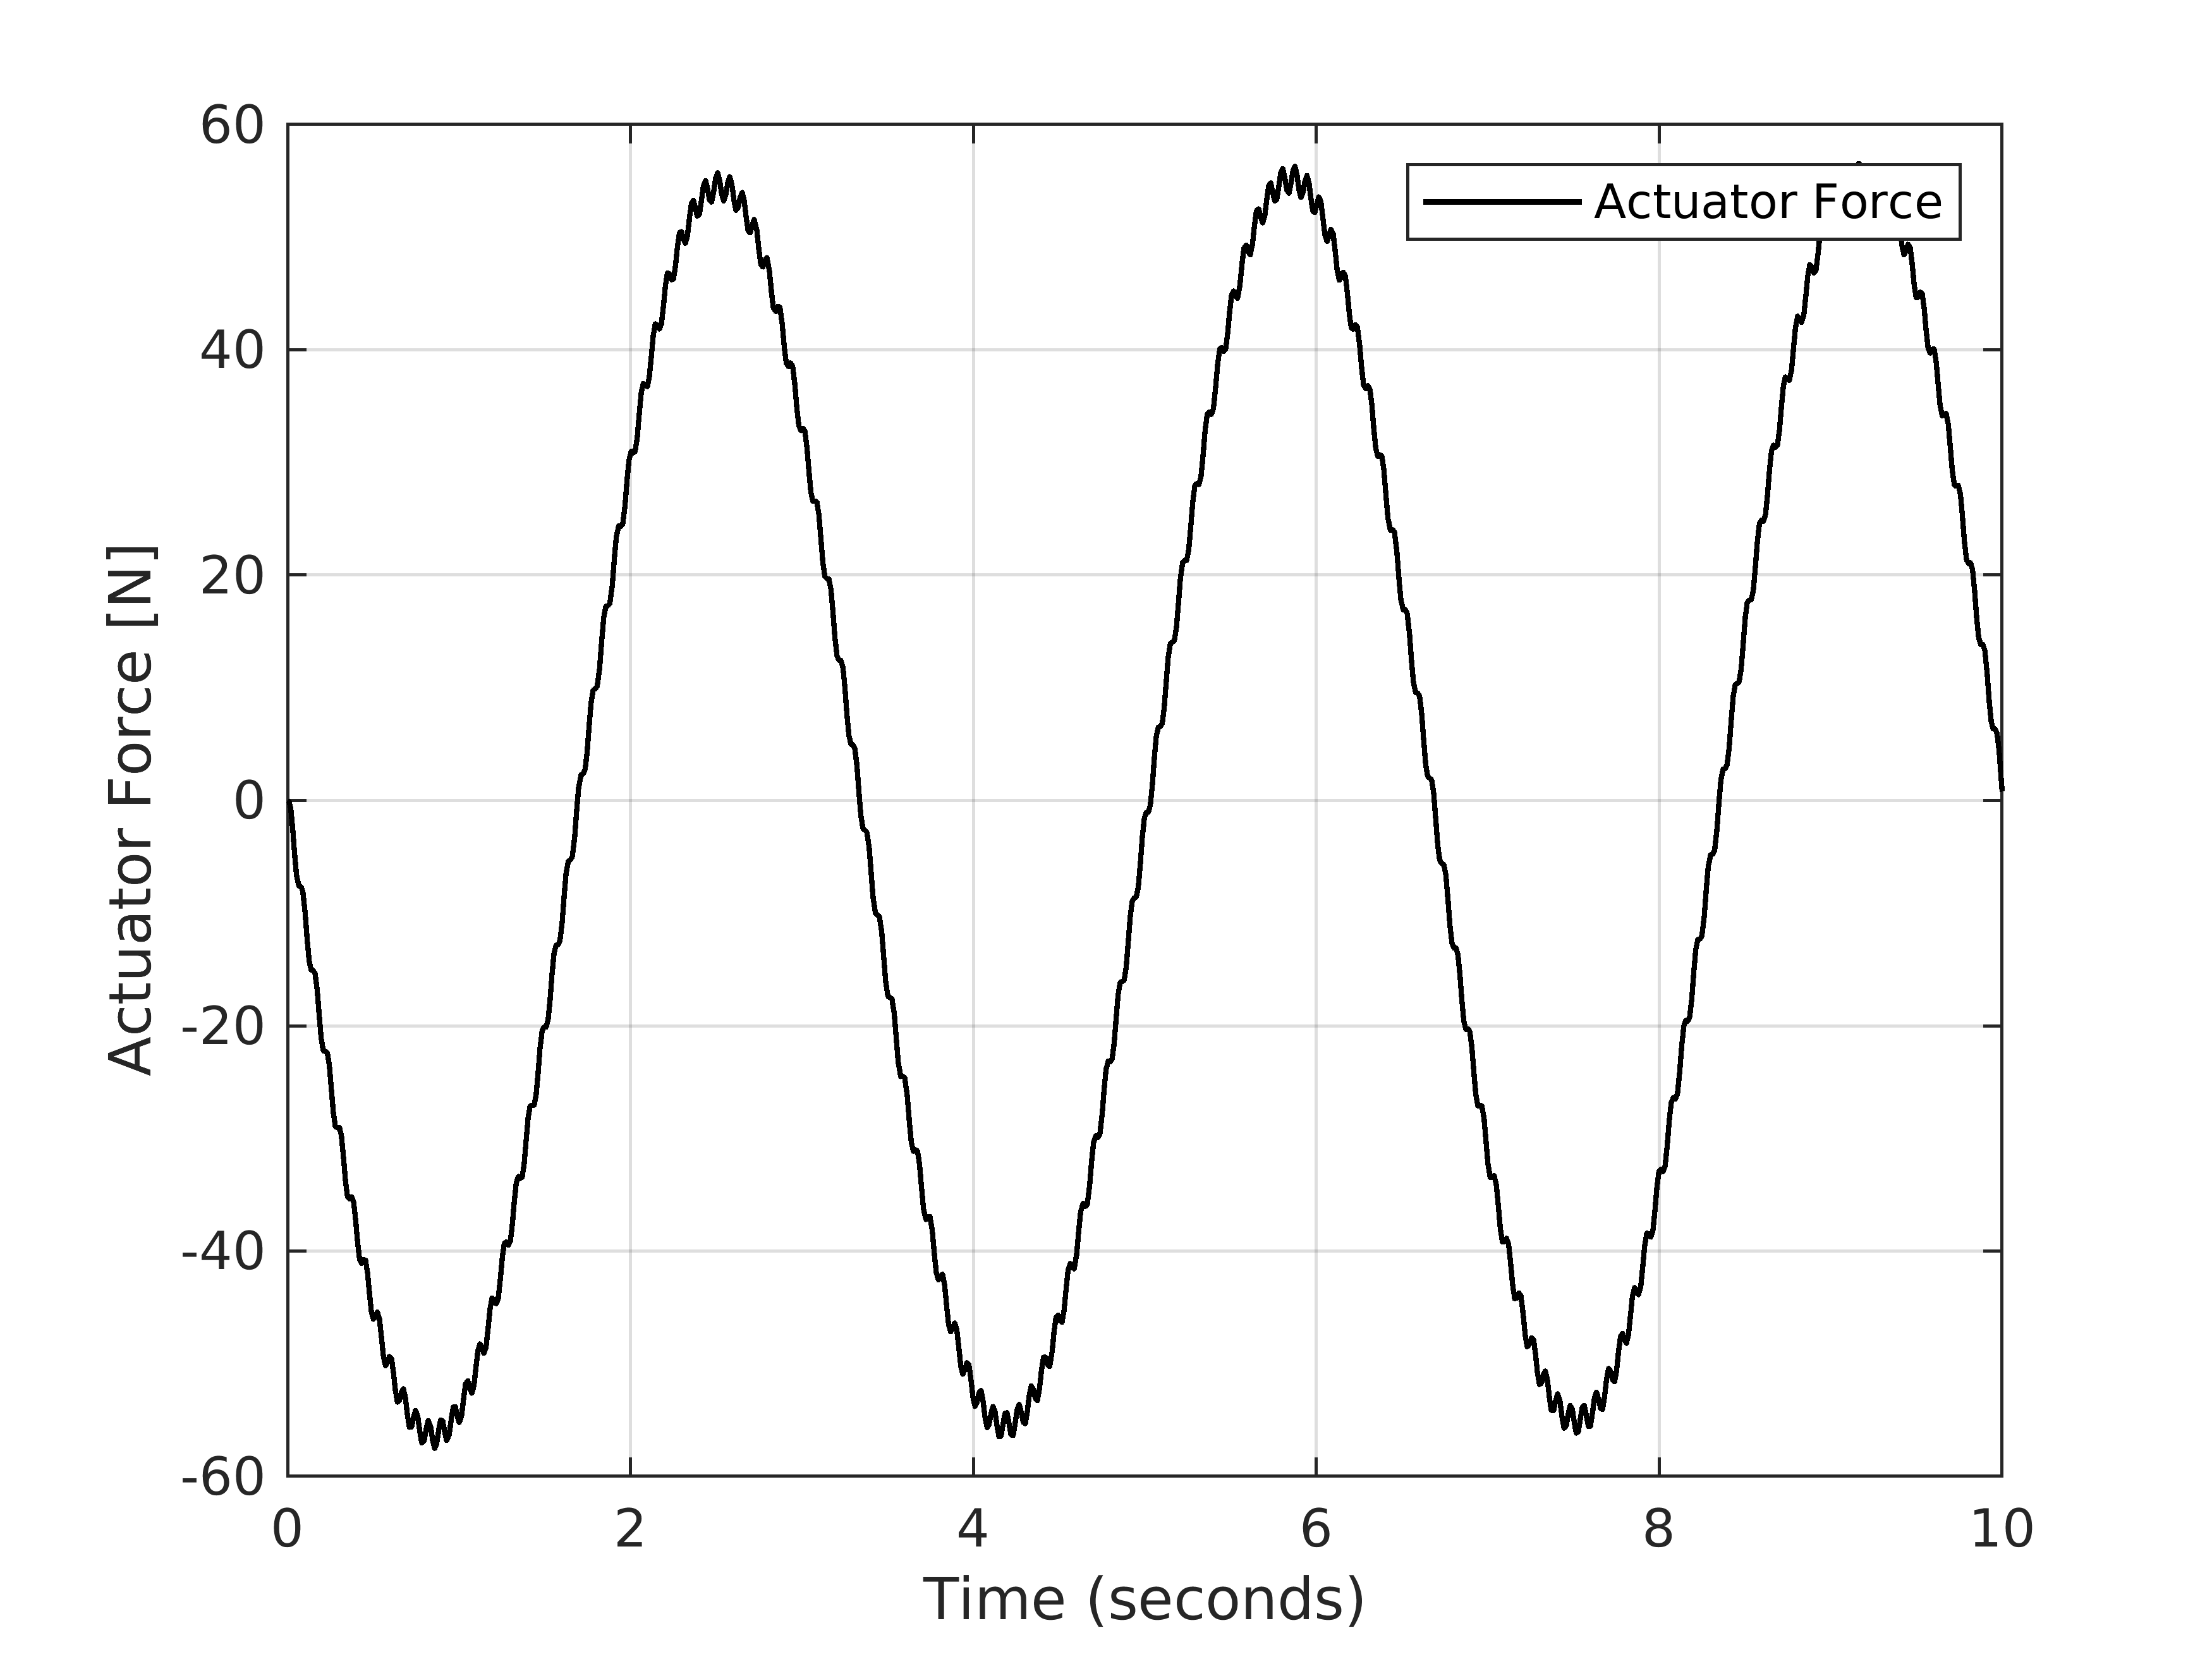
\includegraphics[trim=0cm 2cm 0cm 6cm, clip, width=0.5\textwidth]{force}
	\caption{Force. }
	\label{fig:smc6}
\end{figure}



\newpage
\section{Reinforcement learning}
\subsection{Overview}
Reinforcement learning is a type of machine learning technique where a computer agent learns to perform a task through repeated trial and error interactions with a dynamic environment. This learning approach enables the agent to make a series of decisions that maximize a reward metric for the task without human intervention and without being explicitly programmed to achieve the task.
The key components are:
\begin{itemize}
	\item State (s): Current system observation 
	\item Action (a): Control input applied by the agent 
	\item Reward (r): Feedback signal to guide learning 
	\item Policy : A function mapping states to actions, optimized over time
\end{itemize}

\begin{figure}[H]
	\centering
	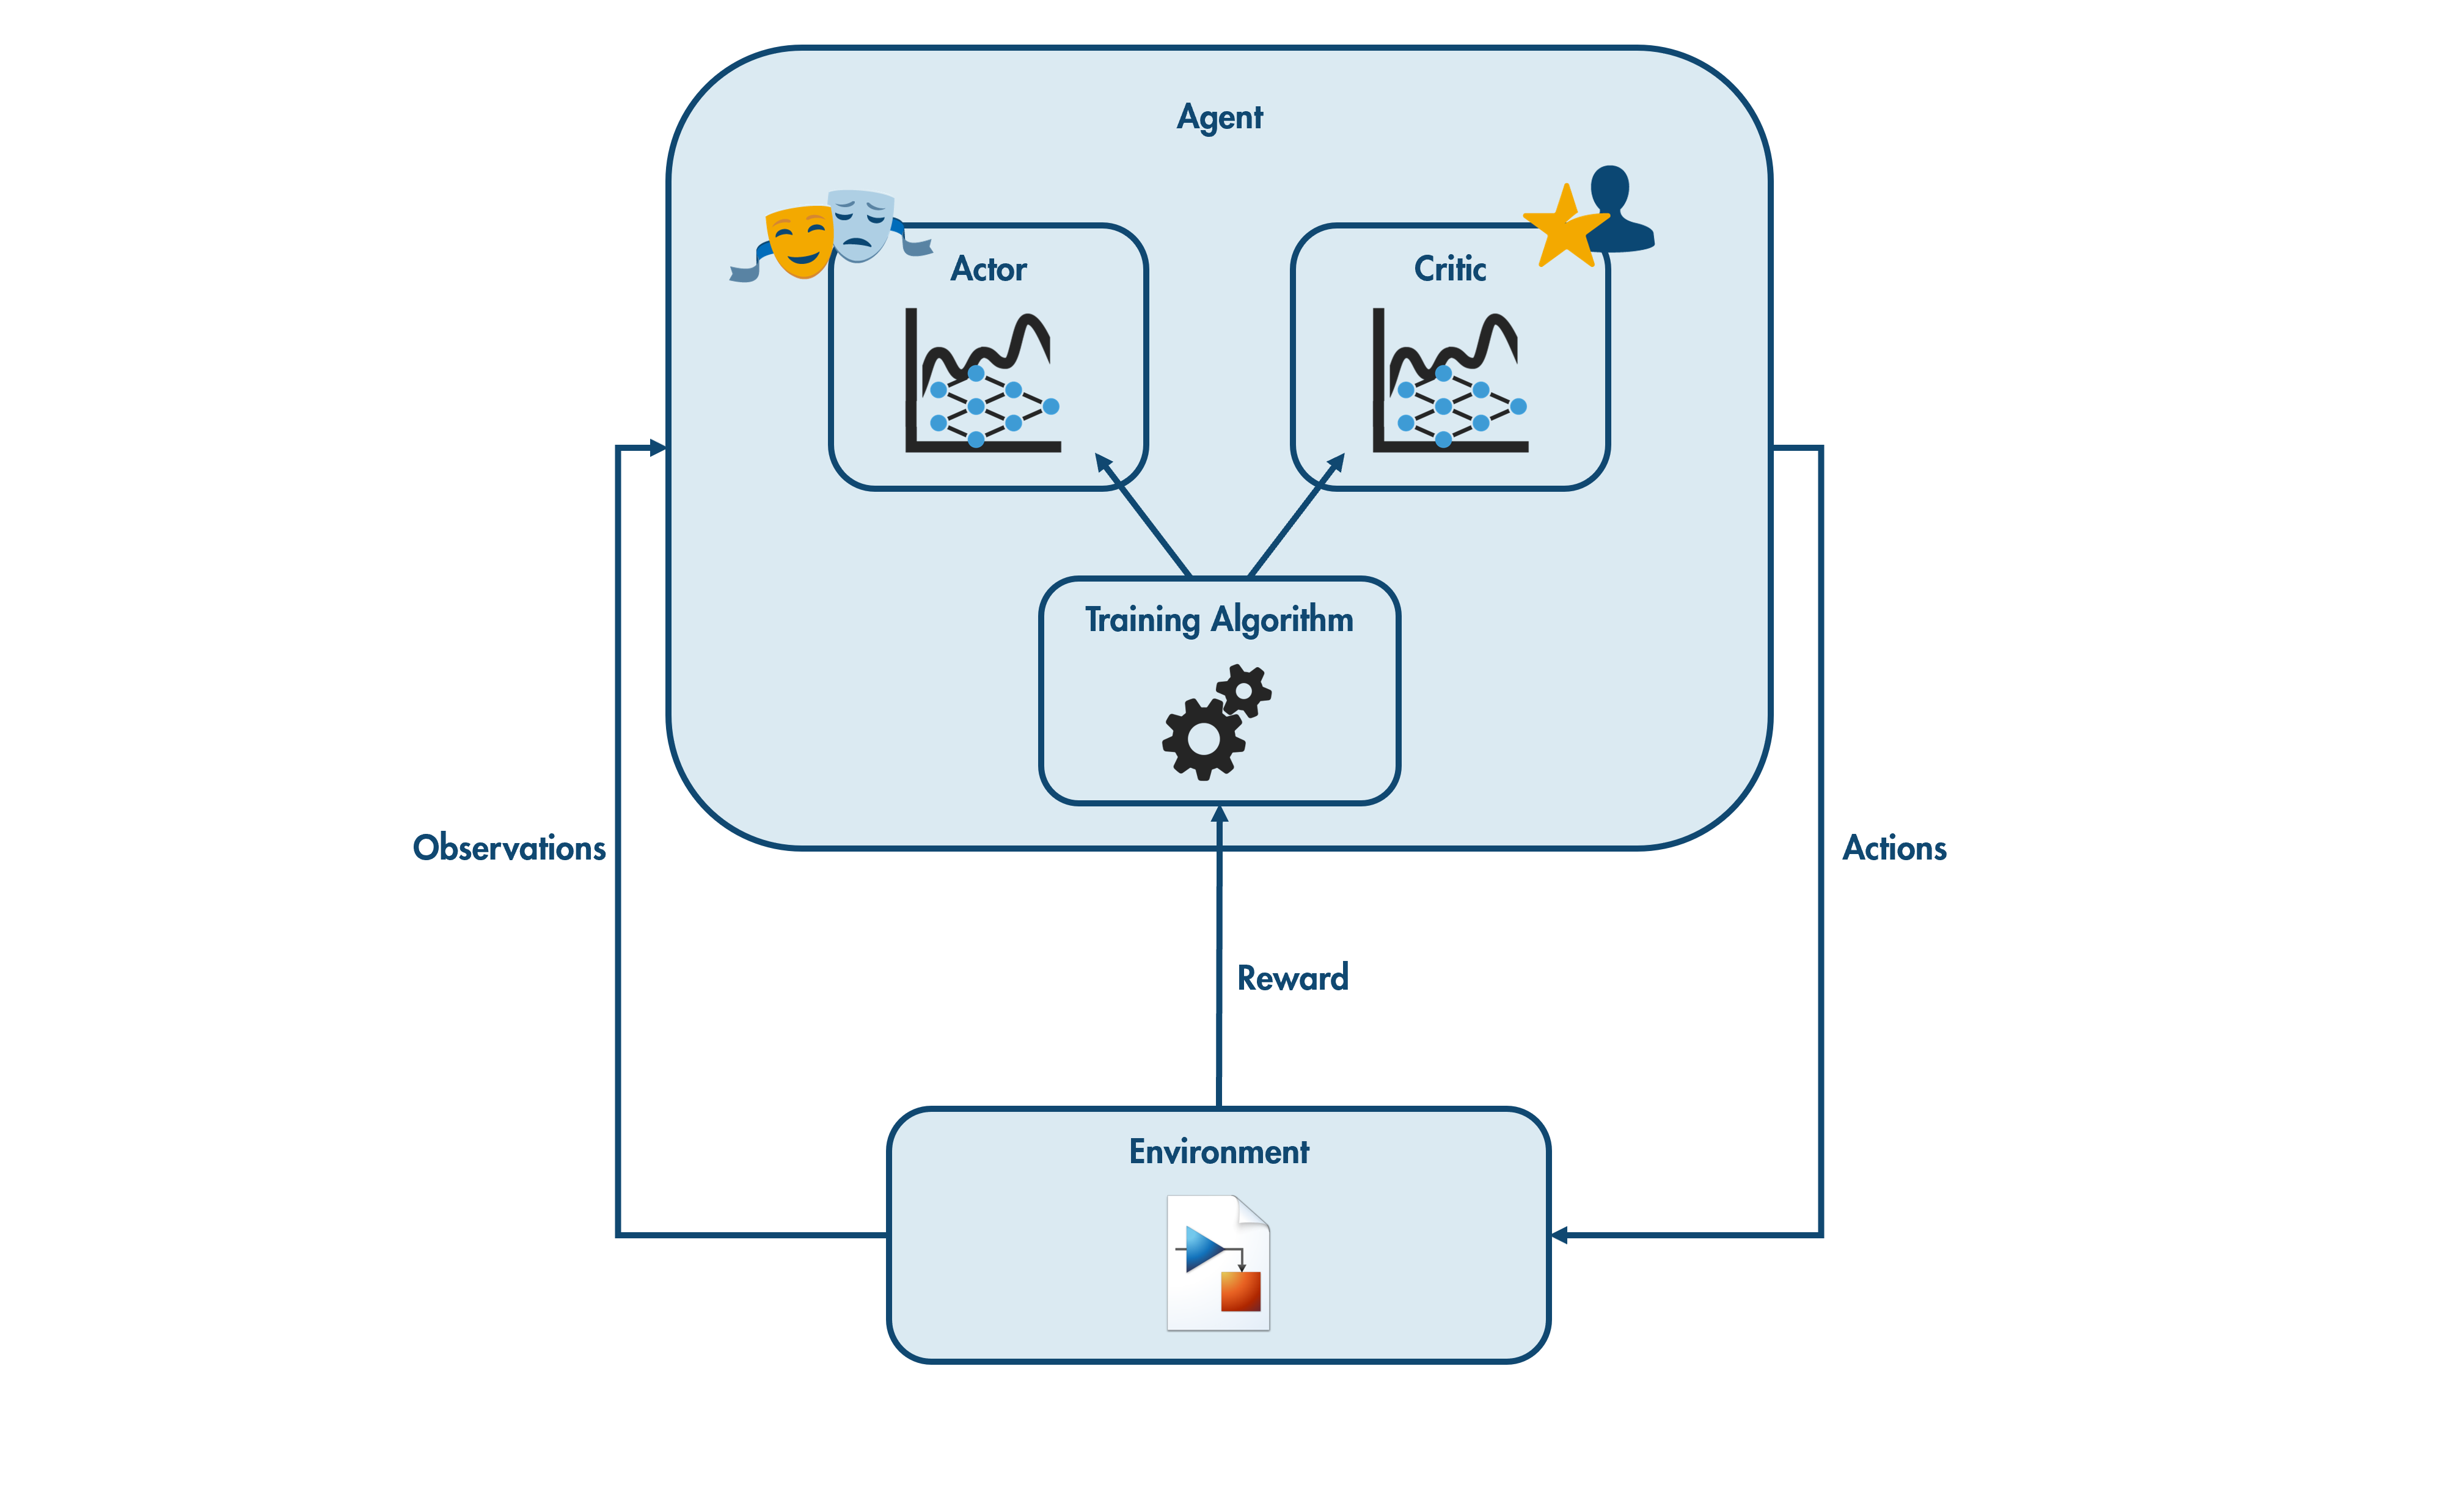
\includegraphics[width=0.8\textwidth]{overview}
	\caption{Reinforcement learning key components. \cite{overview}
	}
\end{figure}

\subsection{Reinforcement learning workflow}
The general workflow for training an agent using reinforcement learning includes the following steps:
\begin{figure}[H]
	\centering
	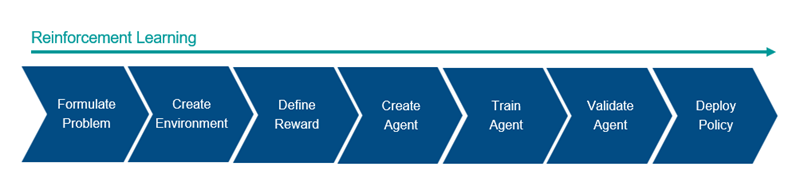
\includegraphics[width=0.8\textwidth]{reinforcement_learning_workflow}
	\caption{RL worlflow. \cite{RL_workflow}
	}
\end{figure}

\newpage
\subsubsection{Create environment }
The environment is modeled using MATLAB/SIMULINK.
\begin{itemize}
	\item Inputst: Road disturbance, control force from the RL agent.
	\item Outputs: Sprung mass displacement, suspension travel, road holding. 
\end{itemize}

Figure\ref{fig:rlm} show the Model used.
\begin{figure}[H]
	\centering
	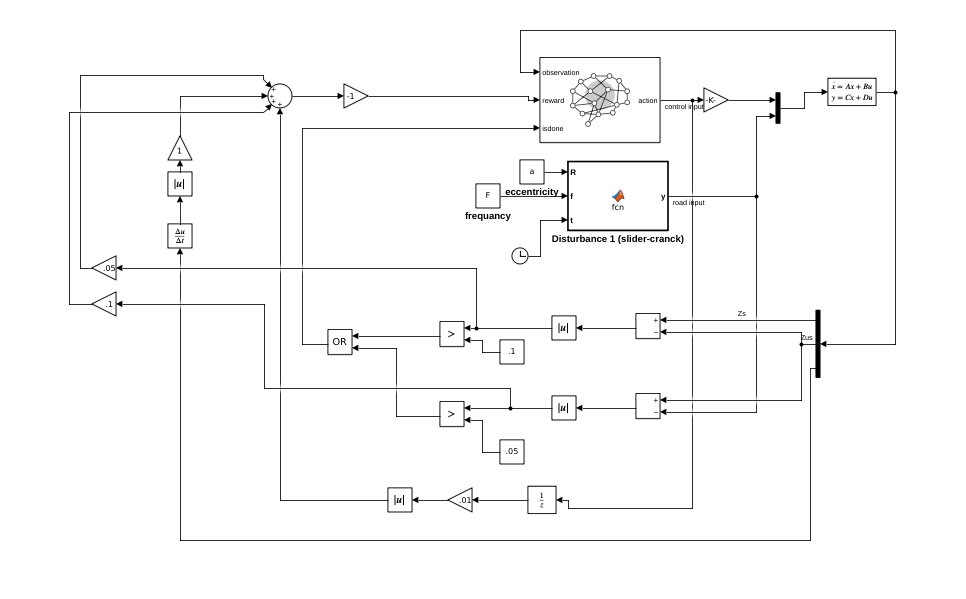
\includegraphics[scale=0.5]{rlsimulink}
	\caption{Reinforcemet learning simulink Model}
	\label{fig:rlm}
\end{figure}

\subsubsection{Design the Reward Function}
Specify the reward signal that the agent uses to measure its performance against the task goals and how to calculate this signal from the environment.

The design objectives are:
\begin{itemize}
	\item Penalize excessive sprung acceleration (improves ride comfort).
	\item Penalize large suspension travel (avoids hitting mechanical limits).
	\item Reward good road holding (minimizing tire deflection).
	\item Penalize excessive control force (reduces energy consumption).
\end{itemize}
\begin{equation}
	R(t) = -\alpha |\ddot{Z_s(t)}| - \beta |Z_s(t) - Z_us| - \gamma |Z_us(t) - Z_r(t)| - \delta |F_c(t)|
\end{equation}

\newpage
\subsubsection{Create agent}
There are many Types of agent choosing between them depends on the nature of our system observation and actions.
\begin{figure}[H]
	\centering
	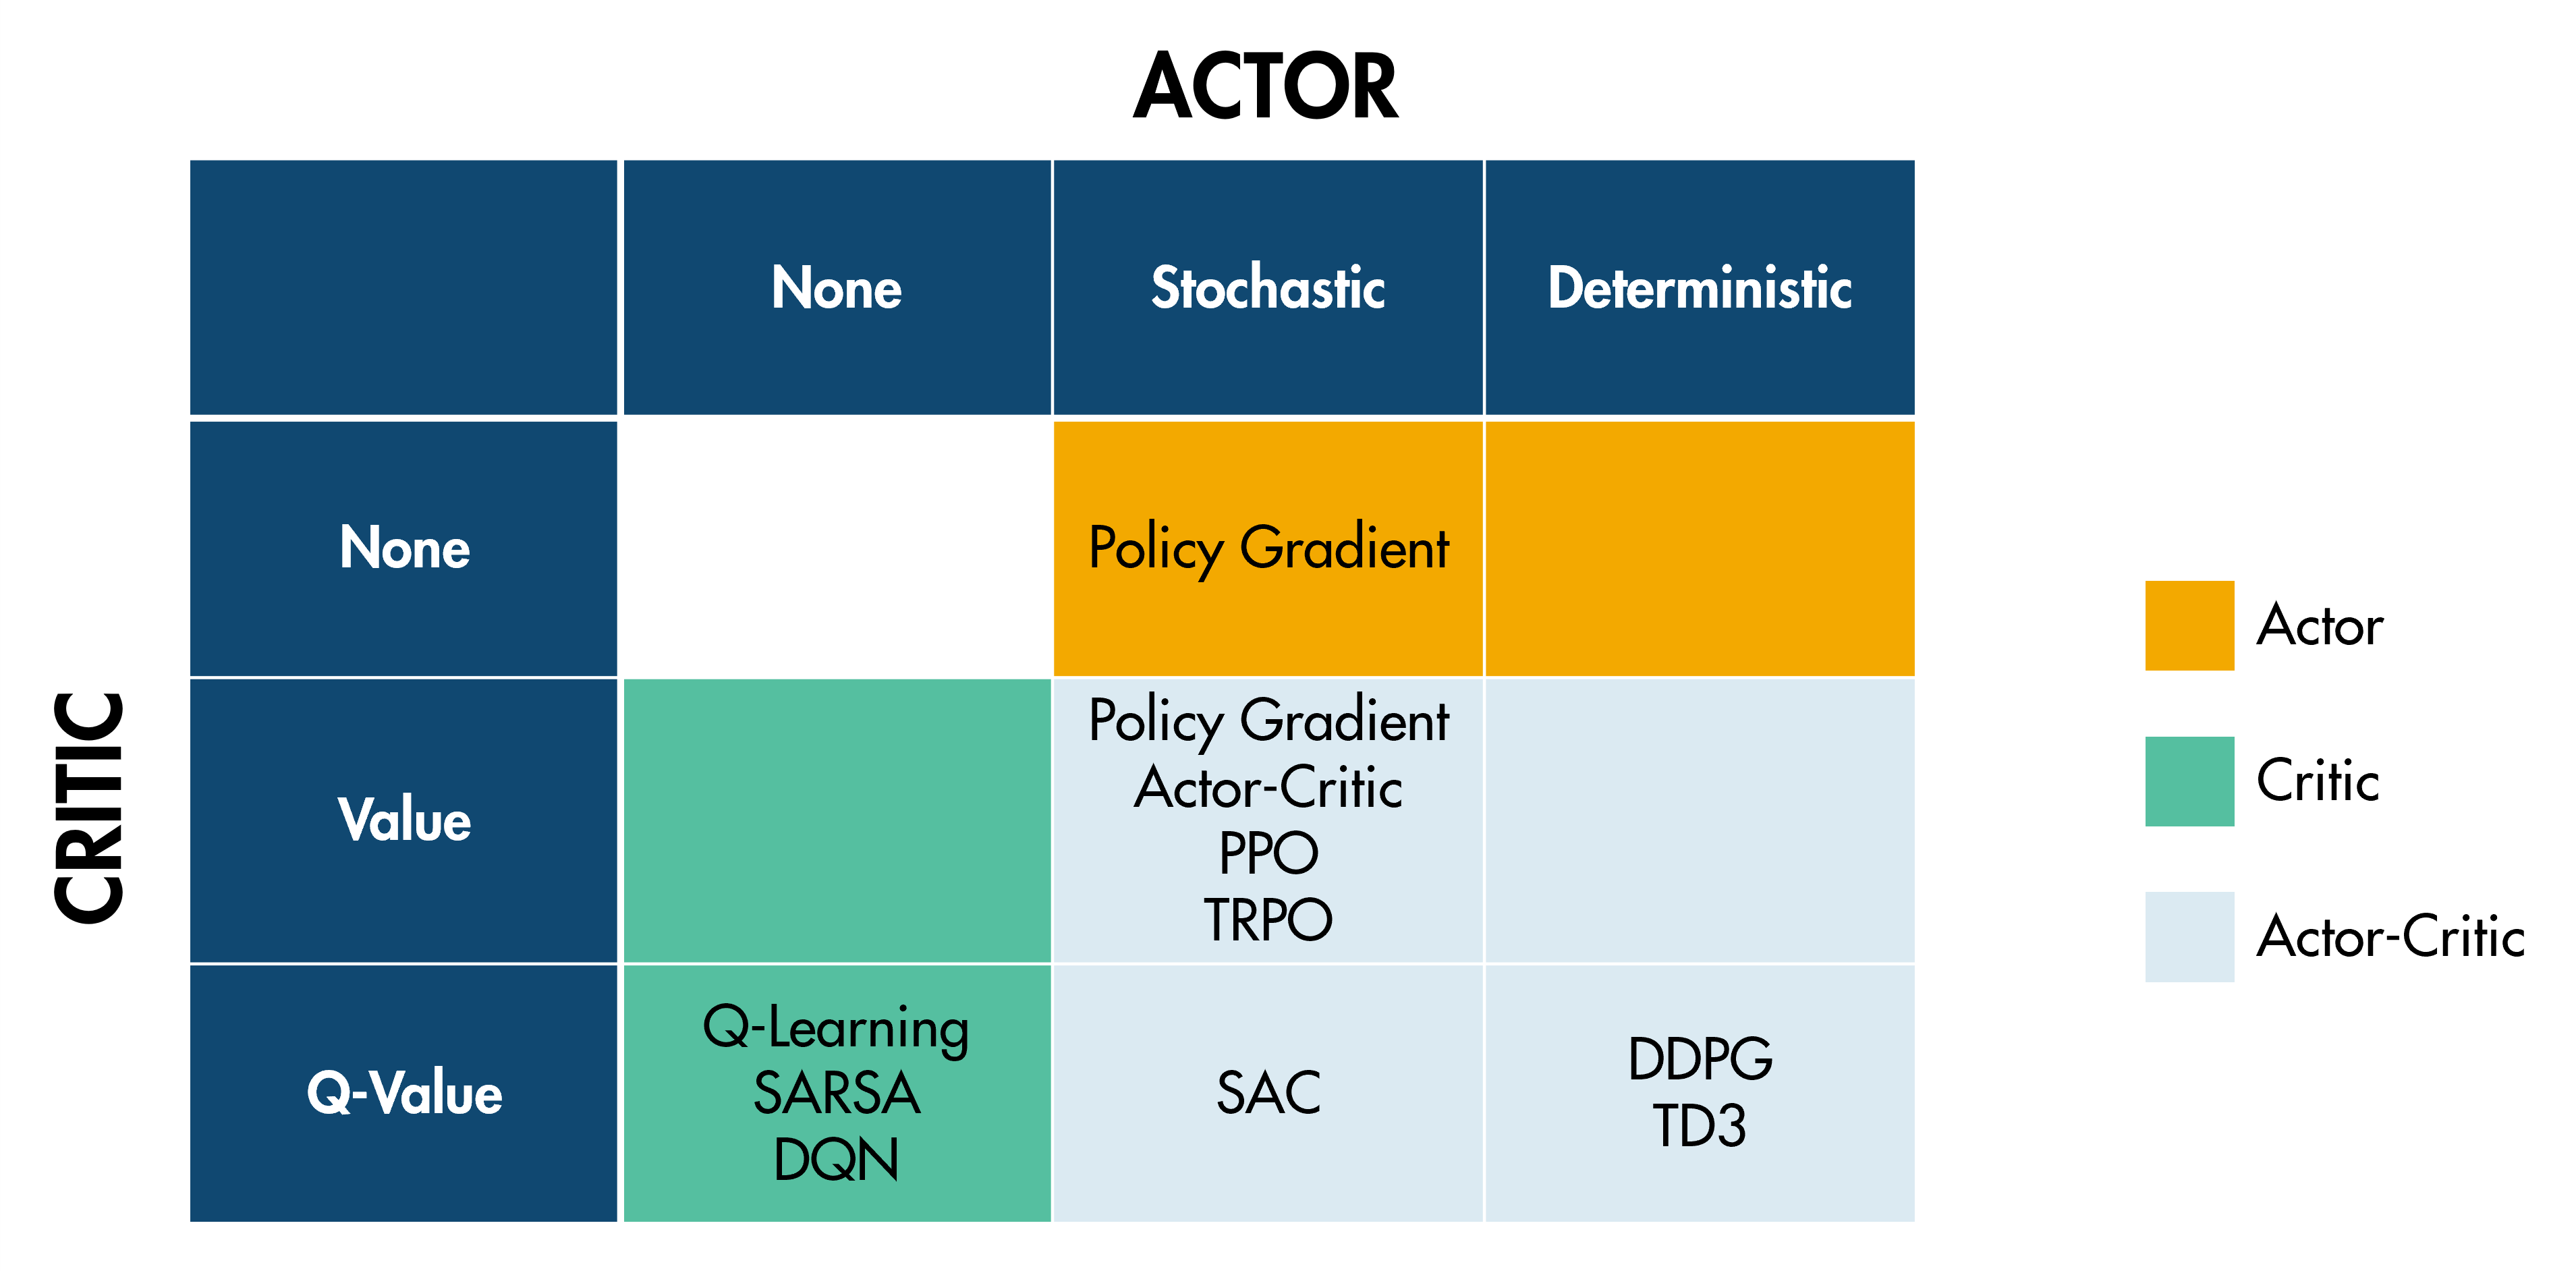
\includegraphics[width=0.8\textwidth]{agents}
	\caption{Reinforcement learning agents. \cite{agents}
	}
\end{figure}

For an active suspension system using DDPG deep Deterministic Policy Gradient is suitable for its continuos nature. It's an extension of the Deterministic Policy Gradient (DPG) method and incorporates deep learning techniques to handle complex environments . It uses two network:
\begin{itemize}
	\item Actor: This network decides which action to take given the current state of the environment.
	\begin{figure}[H]
		\centering
		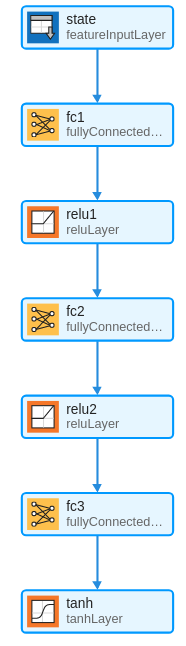
\includegraphics[scale=0.5]{actor}
		\caption{actor network  }
	\end{figure}
	\item Critic: This network evaluates the actions taken by the actor by estimating the Q-value (the expected return from taking a particular action in a given state).
	During training, the Q-values are updated iteratively for each state-action pair based on the agent’s experience using Bellman equation. Over time, this update process allows the agent to learn an optimal policy that maximizes cumulative rewards. The Bellman equation is given by:
	\[ Q(s, a) \leftarrow Q(s, a) + \alpha \left[ r + \gamma \max_{a'} Q(s', a') - Q(s, a) \right] \] where: \begin{itemize} \item \( Q(s, a) \) is the current Q-value for state \( s \) and action \( a \). \item \( \alpha \) is the learning rate. \item \( r \) is the immediate reward after taking action \( a \) in state \( s \). \item \( \gamma \) is the discount factor. \item \( \max_{a'} Q(s', a') \) is the maximum Q-value for the next state \( s' \), over all possible actions \( a' \). \item \( s' \) is the next state. \end{itemize}
	\begin{figure}[H]
		\centering
		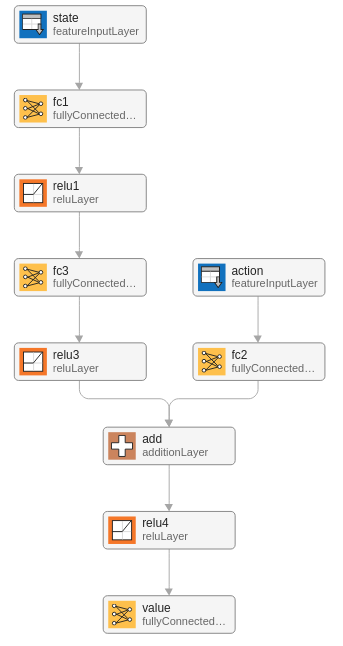
\includegraphics[scale=0.5]{critic}
		\caption{critic network  }
	\end{figure}
\end{itemize}

\newpage
\subsubsection{Train agent}
The agent is trained by interacting with the environment, and the train function will optimize the agent’s policy. The training stats variable will store statistics such as cumulative reward.
\begin{figure}[H]
	\centering
	\includegraphics[scale=0.5]{trainning}
	\caption{training results }
\end{figure}

Training hyper parameters need more tuning and more iterations untill the average reward converge and gives acceptable behavior. Then the tained agent will be validated to make sure it well behave well after deploying in hardware.\newline



The following sections discusses some problems that will arise upon implementing the hardware sensors and actuators for the active system, and how to solve it.

\section {Magnetic Field effect on Sensor Signals}
When an electric motor operates in an active suspension system, it generates a strong magnetic field due to the current flowing through its coils. This magnetic field can significantly affect the electrical signals transmitted through nearby wires, causing interference or distortion in these signals. Several mathematical principles explain this effect.

\subsection{Electromagnetic Induction (Faraday's Law of Induction)}

When a wire is exposed to a changing magnetic field, it induces an electric current in the wire. This phenomenon is known as electromagnetic induction, and it is described by Faraday’s Law of Induction, which states that the induced electromotive force (EMF) (E) is proportional to the rate of change of magnetic flux through the wire. The equation governing this phenomenon is:

\[
E = - \frac{d\Phi_B}{dt}
\]

Where:
\begin{itemize}
	\item \( E \) is the induced electromotive force (EMF).
	\item \( \Phi_B \) is the magnetic flux, calculated as:
	\[
	\Phi_B = B \cdot A
	\]
	\item \( B \) is the magnetic field strength.
	\item \( A \) is the area through which the magnetic flux passes.
\end{itemize}

When the wire is exposed to the magnetic field generated by the motor, the changing magnetic field induces a current in the wire. This induced current can interfere with the original signal being transmitted, leading to signal distortion. In sensitive systems like active suspension, this interference can result in loss of data integrity in the transmitted signals.

\subsection{Effect of the Magnetic Field on Electron Motion in Wires}

The magnetic field acting on a current-carrying wire also exerts a Lorentz force on the moving electrons inside the wire. This force affects the electron motion and can result in changes in current or signal distortion. This force is described by Lorentz's Law:

\[
F = q(v \times B)
\]

Where:
\begin{itemize}
	\item \( F \) is the force acting on the charge \( q \).
	\item \( v \) is the velocity of the charge.
	\item \( B \) is the magnetic field.
\end{itemize}

This force causes the electrons to deviate from their path, which leads to changes in the current flowing through the wire and, consequently, in the electrical signal itself.

\subsection{Electromagnetic Interference (EMI)}

The magnetic field produced by the motor can also cause electromagnetic interference (EMI), which results in the generation of unwanted signals or noise that interferes with the electrical signal transmitted through the wires. Electromagnetic interference can alter both the frequency and amplitude of the signal, leading to signal distortion and loss of signal clarity.

\section{Sensor Accuracy Issues in the System}

Sensors in the active suspension system are crucial for measuring various parameters such as vibration and position. If these sensors are inaccurate, it can directly affect the system's performance. This leads to an incorrect response from the system in controlling the suspension.

\subsection{Measurement Error in Sensors}

Every sensor can have a measurement error due to various factors, such as electromagnetic interference or environmental influences (e.g., temperature and vibration). The relative error in measurements can be expressed using the following equation:

\[
\epsilon = \frac{\Delta S}{S}
\]

Where:
\begin{itemize}
	\item \( \epsilon \) is the relative error in the measurement.
	\item \( \Delta S \) is the change in the actual measurement.
	\item \( S \) is the ideal or reference measurement.
\end{itemize}

The relative error represents the variance between the actual measurements and the ideal measurements. A large relative error indicates that the sensor is inaccurate, which may lead to incorrect readings that negatively impact the system's performance.

\subsection{Impact of Electromagnetic Interference on Sensors}

If sensors are exposed to electromagnetic interference from the motor or other devices within the system, it can lead to an increase in noise within the signal that the sensor measures. Electromagnetic interference from the motor can cause the sensor to record incorrect values. This noise affects the measurement of angles, vibrations, and other critical parameters, leading to an inaccurate system response.

The level of electromagnetic noise caused by multiple sources can be calculated using the following equation:

\[
N = \sum_{i=1}^{n} \frac{1}{r_i^2} \cdot Power_i
\]

Where:
\begin{itemize}
	\item \( N \) is the total noise level caused by multiple sources.
	\item \( r_i \) is the distance between the noise source and the sensor.
	\item \( Power_i \) is the power of the interference from source \( i \).
	\item \( n \) is the number of sources causing interference.
\end{itemize}

If the electromagnetic interference from the motor or other devices is strong, it can cause a significant increase in noise, which adversely affects the accuracy of the sensor measurements.


The magnetic field generated by the motor in an active suspension system induces current in nearby wires, leading to signal distortion due to electromagnetic induction and Lorentz forces. This interference results in noise and loss of data integrity in the transmitted signals. Additionally, sensor inaccuracies due to electromagnetic interference or sensor-related issues can reduce the accuracy of the measurements used for system control. These effects compromise the system's ability to respond accurately.

\section {Solutions to the Effect of Magnetic Field inference}

This section discusses the issue of magnetic field interference caused by motors that can significantly impact signal integrity in sensors used in our system.

Below are some scientifically proven solutions to address this problem:

\subsection {Ferrite Beads}
Ferrite beads are simple yet highly effective electronic components used to suppress electromagnetic interference (EMI) in electrical circuits. They operate by providing high impedance to high-frequency noise while allowing low-frequency signals to pass. Ferrite beads are widely used in applications such as laptop chargers, industrial control systems, and sensitive electronic devices. Studies have shown that ferrite beads can significantly reduce high-frequency noise.



\subsection {Shielded Wires}
Shielded wires are specifically designed to protect internal signals from external electromagnetic interference. These wires are covered with a conductive shield (e.g., metallic braiding or foil), which absorbs or redirects electromagnetic fields. They are essential in applications where signal integrity is critical, such as telecommunications, medical equipment, and industrial machinery.


\subsection {Electronic Filters}
Electronic filters are critical components for managing signal processing and reducing noise. These devices allow specific frequency ranges to pass while attenuating unwanted frequencies. Filters improve signal quality by removing noise caused by EMI or other sources.

\section {Extended Kalman Filter}

\subsection{Overview of the Extended Kalman Filter}

The Extended Kalman Filter (EKF) is an extension of the traditional Kalman Filter (KF) designed to handle nonlinear systems. Unlike the KF, which assumes a linear model, the EKF linearizes the system at each time step using a first-order Taylor expansion around the current state estimate.

\subsection {Key Features of the Extended Kalman Filter}
\begin{itemize}
	\item \textbf{Nonlinear Systems:} The EKF can handle nonlinear system dynamics by linearizing the system around the current estimate.
	\item \textbf{Noise Handling:} The EKF, like the KF, accounts for noise in both the process and measurements.
	\item \textbf{Optimality:} It provides the best possible estimate in a least-squares sense by minimizing the Mean Squared Error (MSE).
\end{itemize}

\subsection {Mathematical Formulation}

1. \textbf{State Equation:}
\[
\mathbf{x}_k = f(\mathbf{x}_{k-1}, \mathbf{u}_k) + \mathbf{w}_{k-1}
\]
where:
\begin{itemize}
	\item \( \mathbf{x}_k \): State vector at time step \( k \).
	\item \( f(\cdot) \): Nonlinear state transition function.
	\item \( \mathbf{w}_{k-1} \): Process noise (assumed to be Gaussian with zero mean and covariance \( \mathbf{Q} \)).
\end{itemize}

2. \textbf{Measurement Equation:}
\[
\mathbf{z}_k = h(\mathbf{x}_k) + \mathbf{v}_k
\]
where:
\begin{itemize}
	\item \( \mathbf{z}_k \): Measurement vector.
	\item \( h(\cdot) \): Nonlinear measurement function.
	\item \( \mathbf{v}_k \): Measurement noise (assumed to be Gaussian with zero mean and covariance \( \mathbf{R} \)).
\end{itemize}

\subsection {Steps in the Extended Kalman Filter}

\subsubsection {1. Initialization}
\begin{itemize}
	\item Initial state estimate: \( \hat{\mathbf{x}}_0 \).
	\item Initial error covariance: \( \mathbf{P}_0 \).
\end{itemize}

\subsubsection {2. Prediction}
\begin{align*}
	\text{Predict the next state:} & \quad \hat{\mathbf{x}}_{k|k-1} = f(\hat{\mathbf{x}}_{k-1|k-1}, \mathbf{u}_k) \\
	\text{Compute the Jacobian of the state transition:} & \quad \mathbf{F}_k = \frac{\partial f}{\partial \mathbf{x}} \bigg|_{\hat{\mathbf{x}}_{k-1|k-1}} \\
	\text{Predict the error covariance:} & \quad \mathbf{P}_{k|k-1} = \mathbf{F}_k \mathbf{P}_{k-1|k-1} \mathbf{F}_k^T + \mathbf{Q}
\end{align*}

\subsubsection{3. Update}
\begin{align*}
	\text{Compute the Jacobian of the measurement function:} & \quad \mathbf{H}_k = \frac{\partial h}{\partial \mathbf{x}} \bigg|_{\hat{\mathbf{x}}_{k|k-1}} \\
	\text{Compute the Kalman Gain:} & \quad \mathbf{K}_k = \mathbf{P}_{k|k-1} \mathbf{H}_k^T (\mathbf{H}_k \mathbf{P}_{k|k-1} \mathbf{H}_k^T + \mathbf{R})^{-1} \\
	\text{Update the state estimate:} & \quad \hat{\mathbf{x}}_{k|k} = \hat{\mathbf{x}}_{k|k-1} + \mathbf{K}_k (\mathbf{z}_k - h(\hat{\mathbf{x}}_{k|k-1})) \\
	\text{Update the error covariance:} & \quad \mathbf{P}_{k|k} = (\mathbf{I} - \mathbf{K}_k \mathbf{H}_k) \mathbf{P}_{k|k-1}
\end{align*}

\section{Application of the Extended Kalman Filter to the Active Suspension Model}

The active suspension system can also be modeled using the EKF approach. Since the suspension system typically includes nonlinearities, the EKF is more suitable than the standard Kalman filter for state estimation.

\subsection {State-Space Representation of the Suspension System}

The state-space representation of the suspension system will have nonlinear functions for both the state transition and the measurement models. Let’s define:

\subsubsection {State Vector (\( \mathbf{x}(t) \))}
\[
\mathbf{x}(t) = \begin{bmatrix}
	z_s(t) \\
	\dot{z}_s(t) \\
	z_u(t) \\
	\dot{z}_u(t)
\end{bmatrix}
\]
where:
\begin{itemize}
	\item \( z_s(t) \): Sprung mass displacement.
	\item \( \dot{z}_s(t) \): Sprung mass velocity.
	\item \( z_u(t) \): Unsprung mass displacement.
	\item \( \dot{z}_u(t) \): Unsprung mass velocity.
\end{itemize}

\subsubsection {Input Vector (\( \mathbf{u}(t) \))}
\[
\mathbf{u}(t) = \begin{bmatrix}
	\dot{Z}_r(t) \\
	F_c(t)
\end{bmatrix}
\]
where:
\begin{itemize}
	\item \( \dot{Z}_r(t) \): Road disturbance velocity.
	\item \( F_c(t) \): Control force from the active suspension.
\end{itemize}

\subsubsection {Measurement Vector (\( \mathbf{y}(t) \))}
\[
\mathbf{y}(t) = \begin{bmatrix}
	z_s(t) \\
	\dot{z}_s(t)
\end{bmatrix}
\]

\subsection {Nonlinear State Transition and Measurement Functions}

Nonlinear State Transition Function \( f(\mathbf{x}, \mathbf{u}) \):
\[
f(\mathbf{x}, \mathbf{u}) = \begin{bmatrix}
	\dot{z}_s(t) \\
	-\frac{K_s}{M_s} z_s(t) - \frac{B_s}{M_s} \dot{z}_s(t) + \frac{K_s}{M_s} z_u(t) + \frac{B_s}{M_s} \dot{z}_u(t) + F_c(t) \\
	\dot{z}_u(t) \\
	\frac{K_s}{M_u} z_s(t) + \frac{B_s}{M_u} \dot{z}_s(t) - \frac{K_s + K_u}{M_u} z_u(t) - \frac{B_s + B_u}{M_u} \dot{z}_u(t)
\end{bmatrix}
\]

Nonlinear Measurement Function \( h(\mathbf{x}) \):
\[
h(\mathbf{x}) = \begin{bmatrix}
	z_s(t) \\
	\dot{z}_s(t)
\end{bmatrix}
\]
